% ============================================================
% MetaDerm-XA — Main LaTeX file for Overleaf
% Copy this entire file as main.tex in Overleaf
% ============================================================

\documentclass[12pt, a4paper]{article}

% --- Packages ---
\usepackage[utf8]{inputenc}
\usepackage[T1]{fontenc}
\usepackage{amsmath, amssymb}
\usepackage{graphicx}
\usepackage{booktabs}
\usepackage{multirow}
\usepackage{xcolor}
\usepackage{hyperref}
\usepackage{cleveref}
\usepackage{algorithm}
\usepackage{algpseudocode}
\usepackage{subcaption}
\usepackage{float}
\usepackage[margin=1in]{geometry}
\usepackage{setspace}
\usepackage{natbib}
\usepackage{lineno}
\usepackage{enumitem}
\usepackage{tikz}
\usetikzlibrary{positioning, arrows.meta, calc, shapes.geometric}

\onehalfspacing
\linenumbers

% Math macros
\newcommand{\prob}{\mathrm{P}}
\newcommand{\sigmoid}{\sigma}
\newcommand{\R}{\mathbb{R}}

\hypersetup{
    colorlinks=true,
    linkcolor=blue!70!black,
    citecolor=green!50!black,
    urlcolor=blue!70!black,
}

\begin{document}

% ============================================================
% TITLE & AUTHORS
% ============================================================
\title{MetaDerm-XA: Field-Wise Metadata Conditioning and Image-Fixed Intervention Analysis for CNN-Based Skin Lesion Classification}

\author{
    Sri Hari Subhash Guptha Gantasala \textsuperscript{1}\thanks{Corresponding author. Email: \texttt{av.sc.u4aie23015@av.students.amrita.edu}},
    Gedela Kiran Kumar\textsuperscript{1}, \\
    Tanneru Preethi\textsuperscript{1},
    Aggnour Abhilash\textsuperscript{1} \\[6pt]
    {\small \textsuperscript{1}Department of Computer Science, Amrita Vishwa Vidyapeetham, Amaravathi, India} \\
}

\date{}
\maketitle

% ============================================================
% ABSTRACT
% ============================================================
\begin{abstract}
\noindent\textbf{Background:} Clinical metadata---patient age, sex, and anatomical site---are central to dermatological diagnosis but most deep learning classifiers either ignore them or fuse them by concatenation, collapsing distinct variables into a single opaque vector.

\noindent\textbf{Method:} MetaDerm-XA encodes each metadata variable as a separate learnable token and conditions CNN spatial features via multi-head cross-attention. This \emph{field-token} design produces a per-variable, spatially resolved attention map ($7{\times}7{\times}4$) and supports an \emph{image-fixed intervention} protocol that sweeps one metadata variable at a time to generate population-level sensitivity curves.

\noindent\textbf{Results:} On the ISIC~2019 official test set (8{,}238 images), field-token cross-attention achieves AUROC 0.896 ($p < 0.001$ vs.\ baseline, DeLong). FiLM reaches 0.904; across five seeds the two are indistinguishable ($\Delta = 0.003$, CI $[-0.003, +0.009]$). Field-token attains the highest single-seed recall (0.855). On ISIC~2020 ($n = 33{,}126$), expressive conditioning (FiLM, field-token) drops 15--17\% in AUROC, whereas simpler methods (concat, cross-attn) and the baseline drop 10--13\%, suggesting overfitting to dataset-specific covariate distributions. Age sweeps across 1{,}327 melanoma cases raise the predicted probability monotonically in 94.3\% of images (mean $\Delta p = 0.274$); site and sex sensitivities are consistent across both architectures.

\noindent\textbf{Conclusion:} Field-token cross-attention matches the best fusion method in discrimination while exposing per-variable spatial routing that FiLM's monolithic transformation cannot provide. The sensitivity protocol is architecture-agnostic and applicable to any metadata-input model. Prospective clinical validation is required before deployment.

\vspace{6pt}
\noindent\textbf{Keywords:} skin lesion classification, melanoma detection, metadata conditioning, cross-attention, explainable AI, model-sensitivity analysis, deep learning
\end{abstract}

% ============================================================
% 1. INTRODUCTION
% ============================================================
\section{Introduction}
\label{sec:intro}

Melanoma accounts for approximately 1.7\% of all cancer diagnoses worldwide~\citep{sung2021global}. Early detection is critical: five-year survival exceeds 99\% for localised disease but drops substantially for distant-stage melanoma~\citep{siegel2023cancer}. Dermoscopy-assisted deep learning systems have demonstrated specialist-level diagnostic accuracy in controlled settings~\citep{esteva2017dermatologist, haenssle2018man}, though recent studies reveal significant performance disparities across skin tones~\citep{groh2024deep}, and their translation to clinical decision support remains an active area of investigation.

In clinical practice, dermatologists do not evaluate dermoscopic images in isolation. Patient metadata---age, biological sex, and the anatomical site of the lesion---are integral to the diagnostic process. Melanoma incidence rises steeply with age~\citep{whiteman2016growing}, exhibits sex-dependent survival disparities~\citep{joosse2011gender}, and has well-characterised anatomical predilections~\citep{elwood1998distribution}. Despite this, the majority of deep learning systems for skin lesion classification operate on image data alone~\citep{brinker2019deep, tschandl2019comparison}, discarding clinically informative metadata that is routinely available at the point of care.

When metadata \emph{is} incorporated, the dominant approach is naive concatenation: the image feature vector and an encoded metadata vector are concatenated and passed through a classification head~\citep{pacheco2020impact, yap2018multimodal}. While simple and effective as a baseline, concatenation offers no mechanism for the metadata to \emph{selectively modulate} spatial image features---for instance, allowing the model to attend differently to a lesion's border irregularity depending on the patient's age. More recently, Feature-wise Linear Modulation (FiLM)~\citep{perez2018film} and its medical imaging derivative MetaBlock~\citep{pacheco2021metablock} have introduced channel-wise affine transformations conditioned on metadata. However, FiLM modulates all channels simultaneously with a single metadata representation, collapsing the distinct contributions of individual clinical variables into an opaque transformation.

A parallel concern is \emph{explainability}. For applicable high-risk AI systems, the EU AI Act~\citep{eu2024aiact} emphasises transparency, information enabling interpretation of outputs, and effective human oversight. A recent systematic review of XAI in dermatology finds that most methods remain limited to post-hoc saliency approaches, with limited rigorous evaluation of clinical utility~\citep{hauser2022skin}. Gradient-weighted Class Activation Mapping (Grad-CAM)~\citep{selvaraju2017grad} provides spatial attention visualisation but is inherently limited to image-based attribution and cannot explain the model's reliance on non-image inputs~\citep{nunnari2021xai}. Counterfactual explanations---``how would the prediction change if this input were different?''---offer a complementary paradigm with roots in causal reasoning~\citep{pearl2009causality, mothilal2020dice}. Recent work has extended counterfactual generation to diffusion-based methods for medical image classification~\citep{atad2024counterfactual}, though these approaches focus on image-level perturbations rather than structured metadata interventions. In the dermatological context, the question \emph{``would this lesion still be classified as melanoma if the patient were 25 instead of 65?''} directly probes whether the model is leveraging metadata in a manner directionally consistent with clinical knowledge.

Two gaps motivate this work. First, existing metadata fusion strategies---concatenation, FiLM, and cross-attention~\citep{erdem2026crossmeta, tranvan2025multimodal}---typically encode metadata as a \emph{monolithic vector}, preventing attribution of routing to individual clinical variables within the fusion mechanism. Second, systematic image-fixed, single-variable sensitivity analysis with population-level aggregation remains uncommon, despite being architecture-agnostic. Each component of our approach (per-variable metadata tokens, image-query/metadata-key attention, model-level perturbation) has appeared in prior work; MetaDerm-XA combines them and evaluates the combination end-to-end.

In this work, we introduce \textbf{MetaDerm-XA} (\textbf{Meta}data-conditioned \textbf{Derm}atology with e\textbf{X}plainable \textbf{A}nalysis), a multimodal classification framework with four contributions:

\begin{enumerate}
    \item \textbf{Field-token cross-attention.} Each metadata variable (age, sex, site, missingness) is encoded as a separate learnable token. Multi-head cross-attention lets the CNN's spatial features attend selectively to each field, producing a $49{\times}4$ routing map decomposed by variable (\Cref{sec:method}).
    
    \item \textbf{Image-fixed intervention protocol.} A single metadata variable is swept across its plausible range while the image and remaining covariates are held constant. Aggregated over the test set, this yields population-level sensitivity curves with bootstrap uncertainty bands (\Cref{sec:counterfactual}). The protocol is architecture-agnostic and applied to both field-token and FiLM.
    
    \item \textbf{Five-model comparison with cross-dataset evaluation.} We compare vision-only, concatenation, single-token cross-attention, FiLM~\citep{perez2018film}, and field-token on ISIC~2019, plus a parameter-matched image-only control. Cross-dataset evaluation on ISIC~2020 reveals that expressive conditioning trades in-distribution gains for larger generalisation drops (\Cref{sec:results}).
    
    \item \textbf{Metadata sensitivity analysis.} Intervention sweeps over 1{,}327 melanoma cases show that both field-token and FiLM learn age, sex, and site dependencies that align directionally with known epidemiological patterns.
\end{enumerate}

% ============================================================
% 2. RELATED WORK
% ============================================================
\section{Related Work}
\label{sec:related}

\subsection{Deep Learning for Skin Lesion Classification}

Convolutional neural networks have achieved dermatologist-level performance on melanoma detection tasks since the landmark study by \citet{esteva2017dermatologist}, who trained an Inception-v3 model on 129{,}450 clinical images. Subsequent work has explored a range of architectures including ResNets~\citep{he2016deep}, EfficientNets~\citep{tan2019efficientnet}, and Vision Transformers~\citep{dosovitskiy2021image}. The ISIC Challenge series~\citep{codella2018skin, tschandl2018ham10000, combalia2019bcn20000} has served as the primary benchmark, with top-performing systems typically employing ensemble methods, aggressive data augmentation, and external pretraining~\citep{gessert2020skin}. Despite achieving high in-distribution accuracy, most systems remain unimodal and do not incorporate the clinical metadata that dermatologists rely on for differential diagnosis.

\subsection{Multimodal Fusion with Clinical Metadata}

Several studies have demonstrated that incorporating patient metadata improves classification accuracy. \citet{pacheco2020impact} systematically evaluated concatenation-based fusion across multiple architectures and reported consistent balanced-accuracy improvements of up to 7\%. \citet{yap2018multimodal} combined dermoscopic images with clinical photographs and metadata through late fusion. More sophisticated approaches include FiLM-based conditioning~\citep{perez2018film}, where metadata generates per-channel scale and shift parameters applied to CNN feature maps. \citet{pacheco2021metablock} introduced MetaBlock for dermatological applications. \citet{gessert2020metadata} further demonstrated metadata-enhanced ensemble EfficientNets for ISIC classification. \citet{tang2022fusionm4net} proposed a multi-stage, multi-modal architecture with dedicated metadata processing streams and decision-level fusion. Recent work has explored cross-attention mechanisms for metadata fusion: \citet{erdem2026crossmeta} proposed a cross-attention mechanism using metadata as queries to attend to visual features. Concurrent and recent work has further explored CNN/metadata cross-attention: \citet{tranvan2025multimodal} employed image-query/metadata-key-value attention for skin-lesion classification and evaluated on HAM10000, ISIC-2019, and PAD-UFES-20. \citet{waseem2026multimodal} used EfficientNet-B0 image tokens with metadata/knowledge-graph keys in an image-query cross-attention framework, and \citet{sonuc2026interpretable} proposed an interpretable multimodal image/metadata fusion approach. Several of these approaches encode the full metadata vector as a \emph{single representation} (e.g., concatenation, standard FiLM, and single-token attention), preventing the model---and the clinician---from attributing model behaviour to individual clinical variables. Recent knowledge-graph-token and field-token methods begin to address this, though systematic per-variable model-sensitivity analysis remains uncommon. Our field-token architecture addresses this by maintaining per-variable tokens throughout the fusion process.

\subsection{Explainability in Medical Image Analysis}

Post-hoc explainability methods for medical imaging predominantly focus on spatial attribution. Grad-CAM~\citep{selvaraju2017grad} and its variants~\citep{chattopadhay2018grad} highlight image regions driving the prediction, while attention rollout~\citep{abnar2020quantifying} provides similar visualisations for transformer architectures. A recent systematic review of XAI in dermatology~\citep{hauser2022skin} finds that spatial attribution remains the dominant approach, with limited rigorous evaluation of whether such explanations improve clinician performance. For multimodal models, spatial explanations alone are insufficient---they cannot explain the influence of non-image inputs~\citep{nunnari2021xai}. Counterfactual explanations~\citep{mothilal2020dice, wachter2018counterfactual} address this gap by answering ``what-if'' questions. In the medical domain, \citet{mertes2022ganterfactual} used GANs to generate counterfactual images, \citet{atad2022chexplaining} applied counterfactual reasoning to chest X-ray images, and more recently \citet{atad2024counterfactual} demonstrated diffusion autoencoder--based counterfactuals for medical image classification. Our image-fixed intervention protocol differs fundamentally from these approaches: rather than generating synthetic images, we intervene on structured metadata inputs, enabling precise, univariate sensitivity analysis that characterises the model's learned reliance on each clinical covariate.

\noindent\textbf{Summary of gaps.} In the literature surveyed here (PubMed and arXiv through September 2026), we did not find a dermatology study combining all of the following: (i)~four explicit tokens for age, sex, anatomical site, and missingness; (ii)~image-token queries attending to those metadata tokens on a CNN spatial backbone; and (iii)~matched ISIC-2019/ISIC-2020 evaluation paired with image-fixed, per-variable sensitivity curves. Metadata-conditioned modulation, skin-lesion cross-attention, field-wise encoding, and fixed-image perturbation have each appeared in prior work. Our intervention results are descriptive probes of model sensitivity, not causal or clinical validation.

\Cref{tab:lit_comparison} summarises the key methodological dimensions across prior work.

\begin{table*}[htbp]
\centering
\caption{Comparison of multimodal skin lesion classification methods. Columns: fusion mechanism, whether metadata fields are encoded as separate tokens ($\checkmark$ = per-variable decomposition), whether per-variable model-sensitivity analysis is reported, number of primary model configurations compared, and cross-dataset evaluation. Ablation counts reflect primary configurations reported in each study; counting conventions differ across papers.}
\label{tab:lit_comparison}
\resizebox{\textwidth}{!}{%
\begin{tabular}{lccccc}
\toprule
Method & Fusion & Per-Variable & Model-Sensitivity & Primary & Cross-Dataset \\
 & Type & Tokens & Analysis & Configs & Evaluation \\
\midrule
Pacheco (2020) & Concat & --- & --- & 2 & --- \\
Gessert (2020) & Concat (ensemble) & --- & --- & 1 & --- \\
Pacheco (2021, MetaBlock) & FiLM & --- & --- & 2 & --- \\
Tang (2022, FusionM4Net) & Multi-stage & --- & --- & $\geq$3$^a$ & --- \\
Erdem (2026) & Cross-Attn (meta$\to$img) & --- & --- & 2 & --- \\
Tran-Van \& Le (2025) & Cross-Attn (img$\to$meta) & --- & --- & 3 & $\checkmark^b$ \\
Waseem (2026) & Cross-Attn + KG tokens & ---$^c$ & --- & 4 & --- \\
\textbf{MetaDerm-XA (Ours)} & \textbf{Field-token cross-attn} & $\checkmark$ & $\checkmark$ & \textbf{5+1}$^d$ & $\checkmark$ \\
\bottomrule
\end{tabular}%
}
\vspace{4pt}
\begin{flushleft}
{\scriptsize $^a$FusionM4Net includes multiple fusion stages and branch predictions; exact ablation counting depends on definition. $^b$Separate benchmark experiments on multiple datasets, not verified frozen-model transfer. $^c$Uses clinical metadata plus knowledge-graph disease tokens; the KG tokens are not per-clinical-variable decomposition. $^d$Five primary models (Baseline, Concat, Cross-Attn, FiLM, Field-Token) plus one parameter-matched image-only control (Baseline-Wide).}
\end{flushleft}
\end{table*}

\Cref{tab:perf_comparison} compares the best reported classification metrics from prior multimodal skin lesion studies against MetaDerm-XA. \textbf{Direct numeric comparison across rows is not valid} because studies differ in dataset, split protocol, task formulation (binary vs.\ multi-class), evaluation protocol (cross-validation vs.\ held-out official test set), and presence of diagnostically ambiguous (UNK) images. In particular, studies reporting cross-validation on the ISIC~2019 \emph{training set} do not evaluate on the 2{,}047 diagnostically unknown (UNK) images present in the official test set, which substantially increases task difficulty. For a same-protocol reference, Gessert et al.\ (2020)---the ISIC~2019 challenge winner---achieved 63.6\% balanced accuracy on the same official test set used by MetaDerm-XA.

\begin{table*}[htbp]
\centering
\caption{Reported classification performance of multimodal skin lesion methods. Metrics are self-reported under heterogeneous protocols; rows are \emph{not} directly comparable. ``---'' = not reported. BA = balanced accuracy. Task: B = binary, M = multi-class. Eval.: CV = cross-validation on training data, HO = held-out official test set, Sep = separate dataset experiment. $\dagger$: proposed method.}
\label{tab:perf_comparison}
\resizebox{\textwidth}{!}{%
\begin{tabular}{llllccccc}
\toprule
Method & Backbone & Dataset & Task & Eval. & AUROC & Acc/BA & Recall & F1 \\
\midrule
Gessert (2020)$^b$ & EfficientNet ens. & ISIC 2019 & M(8) & HO & --- & 0.636 BA & --- & --- \\
Tang (2022) & Multi-stage & ISIC 2019 & M(8) & CV & --- & 0.770 & --- & --- \\
Pacheco (2021) & DenseNet-201 & ISIC 2019 & M(8) & CV & 0.977 & 0.832 BA & --- & --- \\
Sonu\c{c} (2026) & ViT & ISIC 2019 & M(8) & CV & 0.997 & 0.950 & 0.950 & 0.950 \\
\addlinespace
Pacheco (2020)$^a$ & Multi-arch & PAD-UFES-20 & M & CV & --- & +7\% BA & --- & --- \\
Erdem (2026) & ViT & PAD-UFES-20 & B & CV & 0.955 & 0.900 & 0.993 & 0.872 \\
Tran-Van (2025) & CNN & HAM10000 & M(7) & Sep & --- & 0.957 & --- & --- \\
Waseem (2026) & EfficientNet-B0 & HAM10000 & M(7) & Sep & --- & 0.914 & --- & --- \\
\addlinespace
\textbf{Ours (FiLM)}$^\dagger$ & \textbf{EfficientNet-B2} & \textbf{ISIC 2019} & \textbf{B} & \textbf{HO} & \textbf{0.904} & --- & 0.796 & 0.599 \\
\textbf{Ours (Field-Token)}$^\dagger$ & \textbf{EfficientNet-B2} & \textbf{ISIC 2019} & \textbf{B} & \textbf{HO} & 0.896 & --- & \textbf{0.855} & 0.552 \\
\bottomrule
\end{tabular}%
}
\vspace{4pt}
\begin{flushleft}
{\scriptsize $^a$Relative BA improvement over image-only baselines. $^b$ISIC 2019 challenge winner---same official test set as ours (incl.\ 2{,}047 UNK). CV studies on ISIC 2019 training data do not encounter the UNK category, which increases task difficulty. Rows are \emph{not} comparable across datasets, tasks, or evaluation protocols.}
\end{flushleft}
\end{table*}


% ============================================================
% 3. METHODOLOGY
% ============================================================
\section{Methodology}
\label{sec:method}

\Cref{fig:architecture} presents an overview of the proposed field-token cross-attention architecture.
    \begin{figure}[htbp]
        \centering
        \resizebox{0.85\linewidth}{!}{%
        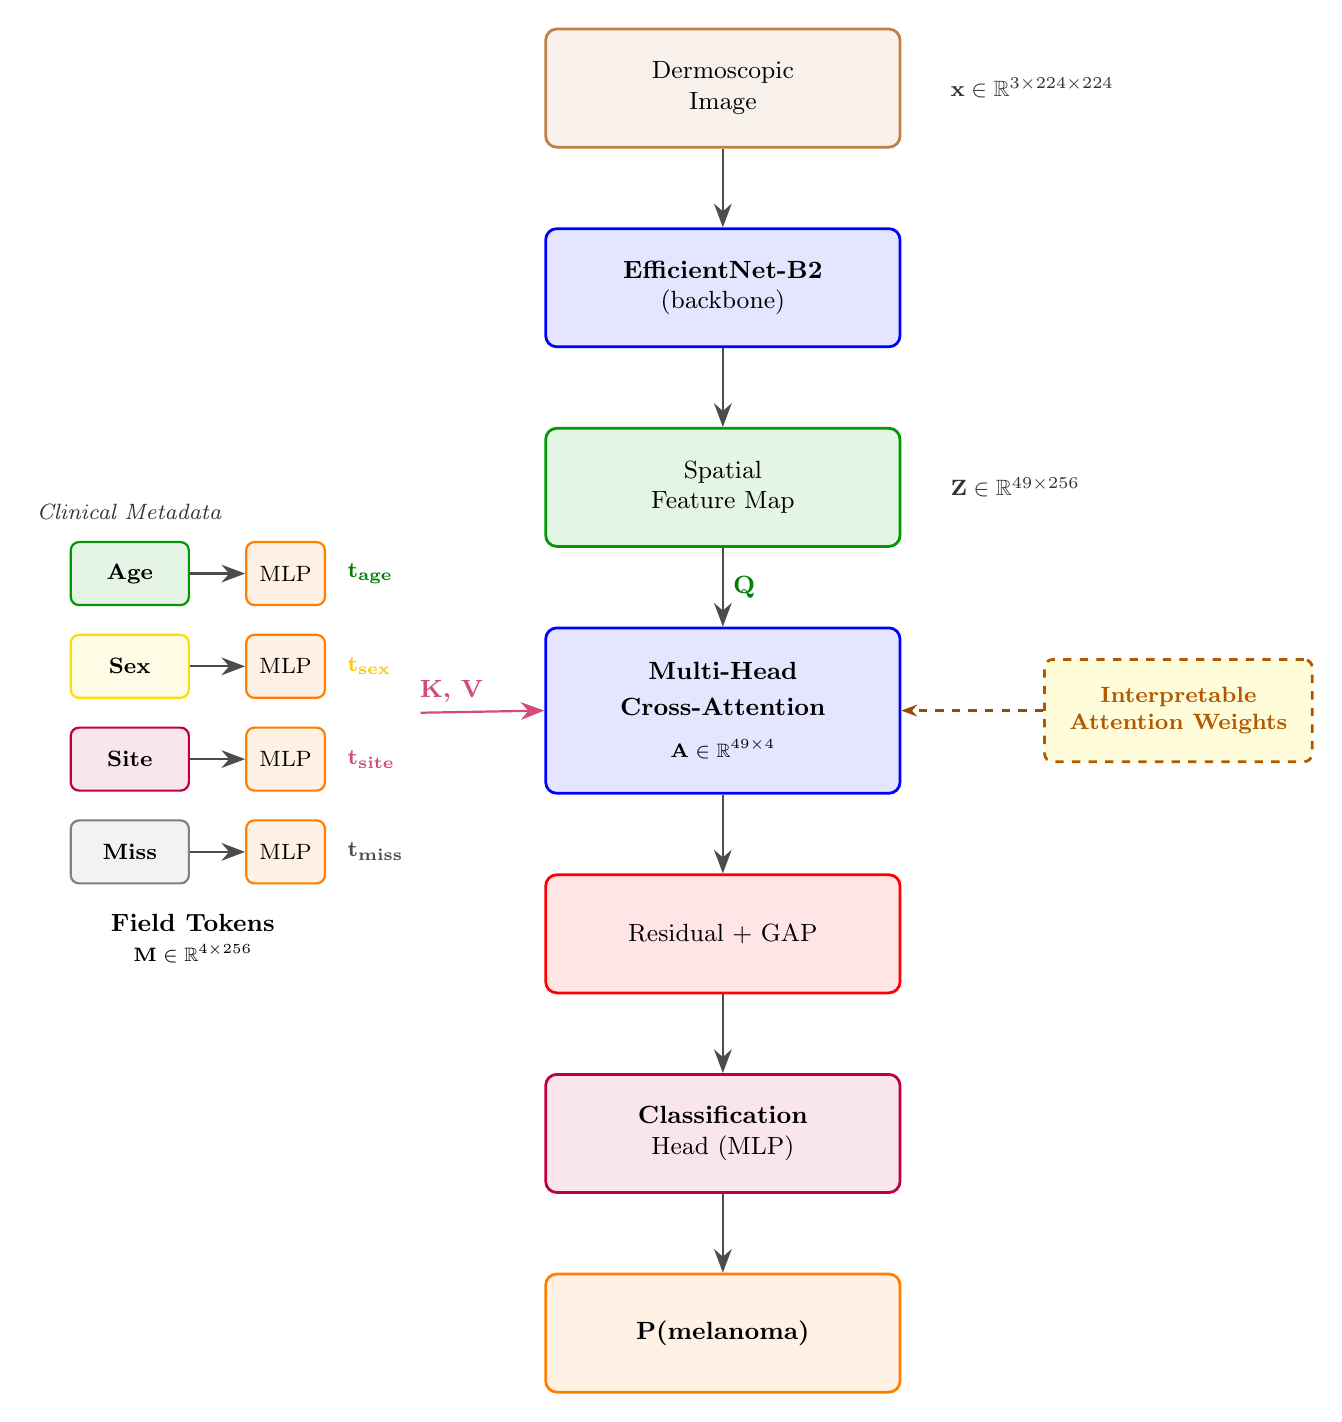
\begin{tikzpicture}[
            node distance=1.0cm and 1.5cm,
            box/.style={rectangle, rounded corners=4pt, draw=#1, fill=#1!10,
                         minimum height=1.5cm, minimum width=4.5cm,
                         text centered, font=\small, line width=1pt},
            smallbox/.style={rectangle, rounded corners=3pt, draw=#1, fill=#1!10,
                             minimum height=0.8cm, minimum width=1.5cm,
                             text centered, font=\footnotesize, line width=0.8pt},
            arr/.style={-{Stealth[length=3mm]}, thick, color=black!70},
            lbl/.style={font=\footnotesize, color=black!80},
            every node/.style={align=center},
        ]
    
        % === MAIN PIPELINE (vertical, top to bottom) ===
        \node[box=brown] (img) {Dermoscopic\\Image};
        \node[lbl, right=0.5cm of img] {$\mathbf{x} \in \R^{3 \times 224 \times 224}$};
    
        \node[box=blue, below=of img] (backbone) {\textbf{EfficientNet-B2}\\(backbone)};
    
        \node[box=green!60!black, below=of backbone] (spatial) {Spatial\\Feature Map};
        \node[lbl, right=0.5cm of spatial] {$\mathbf{Z} \in \R^{49 \times 256}$};
    
        \node[box=blue, below=of spatial, minimum height=2.1cm] (crossattn) {\textbf{Multi-Head}\\[2pt]\textbf{Cross-Attention}\\[4pt]{\scriptsize $\mathbf{A} \in \R^{49 \times 4}$}};
    
        \node[box=red, below=of crossattn] (gap) {Residual + GAP};
    
        \node[box=purple, below=of gap] (cls) {\textbf{Classification}\\Head (MLP)};
    
        \node[box=orange, below=of cls] (output) {\textbf{P(melanoma)}};
    
        % === MAIN ARROWS ===
        \draw[arr] (img) -- (backbone);
        \draw[arr] (backbone) -- (spatial);
        \draw[arr] (spatial) -- node[right, font=\small\bfseries, color=green!50!black] {Q} (crossattn);
        \draw[arr] (crossattn) -- (gap);
        \draw[arr] (gap) -- (cls);
        \draw[arr] (cls) -- (output);
    
        % === METADATA FIELD TOKENS (left side branch) ===
        \node[smallbox=green!60!black, left=4.5cm of crossattn, yshift=1.74cm] (age) {\textbf{Age}};
        \node[smallbox=yellow!80!orange, below=0.35cm of age] (sex) {\textbf{Sex}};
        \node[smallbox=purple, below=0.35cm of sex] (site) {\textbf{Site}};
        \node[smallbox=gray, below=0.35cm of site] (miss) {\textbf{Miss}};
    
        \node[lbl, above=0.15cm of age] {\textit{Clinical Metadata}};
    
        % MLPs
        \node[smallbox=orange, right=0.7cm of age, minimum width=1.0cm] (mlp1) {MLP};
        \node[smallbox=orange, right=0.7cm of sex, minimum width=1.0cm] (mlp2) {MLP};
        \node[smallbox=orange, right=0.7cm of site, minimum width=1.0cm] (mlp3) {MLP};
        \node[smallbox=orange, right=0.7cm of miss, minimum width=1.0cm] (mlp4) {MLP};
    
        \draw[arr] (age) -- (mlp1);
        \draw[arr] (sex) -- (mlp2);
        \draw[arr] (site) -- (mlp3);
        \draw[arr] (miss) -- (mlp4);
    
        % Token labels
        \node[right=0.15cm of mlp1, font=\footnotesize\bfseries, color=green!50!black] {$\mathbf{t}_{\text{age}}$};
        \node[right=0.15cm of mlp2, font=\footnotesize\bfseries, color=yellow!60!orange] {$\mathbf{t}_{\text{sex}}$};
        \node[right=0.15cm of mlp3, font=\footnotesize\bfseries, color=purple!70] {$\mathbf{t}_{\text{site}}$};
        \node[right=0.15cm of mlp4, font=\footnotesize\bfseries, color=gray!60!black] {$\mathbf{t}_{\text{miss}}$};
    
        % Field Tokens label
        \node[below=0.25cm of miss, font=\small\bfseries, xshift=0.8cm] (ftlabel) {Field Tokens\\{\scriptsize $\mathbf{M} \in \R^{4 \times 256}$}};
    
        % Arrow from field tokens to cross-attention (K, V)
        \coordinate (midright) at ($(mlp2.east)!0.5!(mlp3.east)+(1.2, 0)$);
        \draw[arr, purple!70, thick] (midright) -- node[above, near start, font=\small\bfseries, color=purple!70] {K, V} (crossattn.west);
    
        % === INTERPRETABILITY NOTE (right side) ===
        \node[rectangle, rounded corners=3pt, draw=orange!70!black, fill=yellow!15,
              dashed, line width=1pt, minimum width=3.4cm, minimum height=1.3cm,
              font=\footnotesize\bfseries, text=orange!70!black, align=center,
              right=1.8cm of crossattn] (interp) {Interpretable\\Attention Weights};
        \draw[-{Stealth[length=2mm]}, dashed, orange!60!black, thick] (interp.west) -- (crossattn.east);

        \end{tikzpicture}%
        }
    \caption{Overview of the MetaDerm-XA field-token cross-attention architecture. Each metadata variable (age, sex, anatomical site, missingness) is encoded as a separate learnable token via dedicated MLPs. Image spatial features from EfficientNet-B2 serve as queries ($Q$), while the four field tokens serve as keys ($K$) and values ($V$) in multi-head cross-attention, producing a $49 \times 4$ head-averaged field-routing map $\bar{\mathbf{A}}$; faithfulness to the final prediction was not established. Note: the site branch uses a learned embedding lookup rather than an MLP; the figure labels all branches as MLP for visual simplicity.}
    \label{fig:architecture}
\end{figure}

\subsection{Problem Formulation}

Let $\mathbf{x} \in \R^{3 \times H \times W}$ denote a dermoscopic image and $\mathbf{m} = (a, s, \ell, \mathbf{f})$ denote the associated clinical metadata, where $a \in \R$ is the patient's age, $s \in \{\text{male}, \text{female}, \text{unknown}\}$ is the biological sex, $\ell \in \mathcal{L}$ is the anatomical site from a vocabulary of $|\mathcal{L}| = 7$ categories, and $\mathbf{f} \in \{0,1\}^k$ is a binary missingness indicator vector. The task is to learn a function $g(\mathbf{x}, \mathbf{m}) \rightarrow [0, 1]$ that estimates the probability of the lesion being malignant (melanoma).

\subsection{Vision Backbone}

We employ EfficientNet-B2~\citep{tan2019efficientnet} pretrained on ImageNet as the shared vision backbone across all models. The classification head and global pooling layer are removed, yielding spatial feature maps $\mathbf{F} \in \R^{B \times C \times H' \times W'}$, where $C = 1408$, $H' = W' = 7$ for $224 \times 224$ input images. For models requiring token sequences, the spatial dimensions are flattened and linearly projected:
\begin{equation}
    \mathbf{Z} = \text{Proj}(\text{Flatten}(\mathbf{F})) \in \R^{B \times N \times D}
\end{equation}
where $N = H' \times W' = 49$ spatial tokens and $D = 256$ is the shared feature dimension.

\subsection{Metadata Encoding Strategies}

\subsubsection{Shared Metadata Encoder (Concat, Cross-Attn, FiLM)}

For the concatenation, single-token cross-attention, and FiLM models, all metadata variables are encoded jointly through a shared metadata encoder:
\begin{equation}
    \mathbf{v}_{\text{meta}} = \text{MLP}\left([\mathbf{c}; \mathbf{e}_\ell]\right) \in \R^{D}
\end{equation}
where $\mathbf{c} = [a_{\text{norm}},\, \mathbf{s}_{\text{ohe}},\, f_a] \in \R^5$ concatenates the $z$-normalised age ($\R^1$), three-element one-hot sex encoding for male/female/unknown ($\R^3$; unknown sex is encoded as $[0,0,1]$), and a binary age-missingness indicator $f_a \in \{0,1\}$ flagging imputed age values. Sex missingness is encoded implicitly through the unknown category, and site missingness is represented by an explicit unknown embedding, $\mathbf{e}_\ell \in \R^{16}$ is a learned anatomical site embedding, and $[\cdot ; \cdot]$ denotes concatenation.

\subsubsection{Field-Token Metadata Encoder}

The field-token architecture encodes each metadata variable as a \emph{separate} learnable token:
\begin{align}
    \mathbf{t}_{\text{age}} &= \text{MLP}_{\text{age}}(a_{\text{norm}}) \in \R^D \label{eq:t_age} \\
    \mathbf{t}_{\text{sex}} &= \text{MLP}_{\text{sex}}(\mathbf{s}_{\text{ohe}}) \in \R^D \quad (\mathbf{s}_{\text{ohe}} \in \R^3) \\
    \mathbf{t}_{\text{site}} &= \text{Embed}_{\text{site}}(\ell) \in \R^D \\
    \mathbf{t}_{\text{miss}} &= \text{MLP}_{\text{miss}}(f_a) \in \R^D \label{eq:t_miss}
\end{align}
These four tokens are stacked into a metadata token matrix:
\begin{equation}
    \mathbf{M} = [\mathbf{t}_{\text{age}};\ \mathbf{t}_{\text{sex}};\ \mathbf{t}_{\text{site}};\ \mathbf{t}_{\text{miss}}] \in \R^{B \times 4 \times D}
    \label{eq:field_tokens}
\end{equation}

This decomposition is the key architectural distinction from prior work. By maintaining separate tokens, the cross-attention mechanism can attend to each metadata field independently at each spatial location, and the model-sensitivity protocol can intervene on individual variables while preserving the others.

\subsection{Fusion Mechanisms}

\subsubsection{Concatenation Fusion (Baseline)}

The pooled image feature vector and metadata vector are concatenated and passed through a classification MLP:
\begin{equation}
    \hat{y} = \sigmoid\!\left(\text{MLP}_{\text{cls}}\left([\text{GAP}(\mathbf{F});\ \mathbf{v}_{\text{meta}}]\right)\right)
\end{equation}

\subsubsection{FiLM Conditioning}

Feature-wise Linear Modulation~\citep{perez2018film} generates per-channel scale ($\gamma$) and shift ($\beta$) parameters from the metadata:
\begin{equation}
    \gamma = \sigmoid(\mathbf{W}_\gamma \mathbf{v}_{\text{meta}}),\quad
    \beta = \mathbf{W}_\beta \mathbf{v}_{\text{meta}}
\end{equation}
\begin{equation}
    \tilde{\mathbf{F}} = \gamma \odot \mathbf{F} + \beta
\end{equation}
where $\gamma, \beta \in \R^C$ are broadcast across spatial dimensions. The sigmoid activation constrains $\gamma \in (0,1)^C$, making this a restricted FiLM variant that applies fractional scaling rather than unconstrained affine transformation. The modulated features are then globally average-pooled and classified via $\hat{y} = \sigmoid(\text{MLP}_{\text{cls}}(\text{GAP}(\tilde{\mathbf{F}})))$.

\subsubsection{Single-Token Cross-Attention}

The metadata vector $\mathbf{v}_{\text{meta}}$ is treated as a single key--value token. Image spatial tokens $\mathbf{Z}$ serve as queries:
\begin{equation}
    \text{Attn}(\mathbf{Z}, \mathbf{v}_{\text{meta}}) = \text{softmax}\!\left(\frac{\mathbf{Z}\mathbf{W}_Q (\mathbf{v}_{\text{meta}}\mathbf{W}_K)^\top}{\sqrt{D/h}}\right) \mathbf{v}_{\text{meta}}\mathbf{W}_V
\end{equation}
where $h$ is the number of attention heads. Note that with a single key/value token, the softmax weight is identically one at every spatial location; this control therefore provides a spatially constant metadata-dependent residual shift and lacks field-wise or spatial routing. The output is residually added to $\mathbf{Z}$, globally averaged, and classified.

\subsubsection{Field-Token Cross-Attention (Proposed)}

The field-token matrix $\mathbf{M} \in \R^{B \times 4 \times D}$ serves as keys and values, while image tokens $\mathbf{Z} \in \R^{B \times 49 \times D}$ serve as queries:
With $H=8$ heads and $d_h = D/H = 32$, for each head $h = 1, \ldots, H$:
\begin{align}
    \mathbf{Q}^{(h)} &= \mathbf{Z}\mathbf{W}_Q^{(h)} \in \R^{B \times 49 \times d_h}, \quad
    \mathbf{K}^{(h)} = \mathbf{M}\mathbf{W}_K^{(h)} \in \R^{B \times 4 \times d_h}, \quad
    \mathbf{V}^{(h)} = \mathbf{M}\mathbf{W}_V^{(h)} \in \R^{B \times 4 \times d_h} \\
    \mathbf{A}^{(h)} &= \text{softmax}\!\left(\frac{\mathbf{Q}^{(h)}(\mathbf{K}^{(h)})^\top}{\sqrt{d_h}}\right) \in \R^{B \times 49 \times 4}
    \label{eq:attention_weights}
\end{align}
The multi-head output is concatenated and projected:
\begin{equation}
    \tilde{\mathbf{Z}} = \mathbf{Z} + \text{Concat}_{h=1}^{H}\!\left(\mathbf{A}^{(h)} \mathbf{V}^{(h)}\right) \mathbf{W}_O
    \label{eq:field_token_output}
\end{equation}
where $\mathbf{W}_O \in \R^{D \times D}$. For visualisation, we report the head-averaged attention map $\bar{\mathbf{A}} = H^{-1}\sum_{h=1}^{H} \mathbf{A}^{(h)} \in \R^{B \times 49 \times 4}$. Each entry $\bar{A}_{i,j}$ quantifies how much spatial location $i$ attends to metadata field $j$ on average across heads. This yields a $49 \times 4$ routing map per image that can be reshaped to $7 \times 7 \times 4$ for spatial visualisation. We note that attention weights describe routing allocation and are not validated as faithful feature-importance indicators without additional faithfulness testing.

The fused representation is globally average-pooled and passed through a classification head:
\begin{equation}
    \hat{y} = \sigmoid\!\left(\text{MLP}_{\text{cls}}\!\left(\text{GAP}(\tilde{\mathbf{Z}})\right)\right)
\end{equation}

\noindent\textbf{Spatial interpretation under GAP.} Because GAP immediately follows the cross-attention residual, the classifier receives $\text{GAP}(\tilde{\mathbf{Z}}) = \bar{\mathbf{Z}} + \text{Concat}_h(\sum_j r_j^{(h)} \mathbf{v}_j^{(h)}) \mathbf{W}_O$, where $r_j^{(h)} = 49^{-1}\sum_i a_{ij}^{(h)}$ are mean field weights. The explicit spatial arrangement of attention is not preserved under this linear pooling. However, nonlinear query dependence survives: the mean of attention-weighted outputs generally differs from the attention at the mean query, so the spatial attention distribution does affect the pooled result. We note that the restricted FiLM variant also commutes with GAP: $\text{GAP}(\gamma \odot \mathbf{F} + \beta) = \gamma \odot \text{GAP}(\mathbf{F}) + \beta$. Claims about fine-grained spatial advantages of field-token attention over FiLM should therefore be qualified.

\subsection{Training Protocol}

All models share the same training configuration for fair comparison:
\begin{itemize}
    \item \textbf{Loss:} Binary cross-entropy with class-weight $w_+ = 5.0$ to address melanoma imbalance
    \item \textbf{Optimiser:} AdamW~\citep{loshchilov2019decoupled} ($\eta = 3 \times 10^{-5}$, weight decay $= 5 \times 10^{-4}$)
    \item \textbf{Scheduler:} Cosine annealing over 25 epochs
    \item \textbf{Regularisation:} Dropout ($p = 0.4$)
    \item \textbf{Augmentation:} Horizontal/vertical flips, random rotation ($\pm 90^\circ$), colour jitter (brightness, contrast, saturation), coarse dropout
    \item \textbf{Mixed precision:} Automatic mixed precision (AMP) for training efficiency
    \item \textbf{Early stopping:} Patience of 8 epochs monitoring validation AUROC
    \item \textbf{Input resolution:} $224 \times 224$ pixels, normalised to ImageNet statistics
\end{itemize}

\Cref{tab:params} reports the trainable parameter counts. All metadata-conditioned models are comparable in capacity (8.18M--8.96M). A parameter-matched image-only control (Baseline-Wide, 9.02M) is evaluated in \Cref{tab:multi_seed} to confirm that observed performance differences arise from the conditioning mechanism rather than model capacity.

\begin{table}[htbp]
\centering
\caption{Trainable parameter counts for all models. All share the EfficientNet-B2 backbone (7.70M parameters).}
\label{tab:params}
\begin{tabular}{lcc}
\toprule
Model & Total Parameters & Fusion-Specific \\
\midrule
Baseline & 7.88M & 0.18M \\
Concat Fusion & 8.18M & 0.48M \\
Cross-Attn (1-token) & 8.91M & 1.21M \\
FiLM & 8.84M & 1.14M \\
Field-Token (proposed) & 8.96M & 1.25M \\
\bottomrule
\end{tabular}
\end{table}

\subsection{Data Preprocessing}

Age values are $z$-normalised using training-set statistics ($\mu = 54.2$, $\sigma = 18.1$). Biological sex is one-hot encoded (male, female), and anatomical site is mapped to an integer index for embedding lookup. Missing age values are imputed with the training-set median and flagged with a binary indicator ($f_a = 1$). Missing sex is not mode-imputed; instead, it is mapped to an explicit unknown category and encoded as $[0, 0, 1]$ in the three-element one-hot vector. Missing anatomical site is similarly mapped to an unknown embedding category. This design allows the model to distinguish observed from missing metadata without conflating absent data with the most frequent value.

% ============================================================
% 4. IMAGE-FIXED MODEL-SENSITIVITY PROTOCOL
% ============================================================
\section{Image-Fixed Model-Sensitivity Protocol}
\label{sec:counterfactual}

\subsection{Image-Fixed Interventions}

Given a trained model $g(\mathbf{x}, \mathbf{m})$, we define an \emph{image-fixed model-level intervention} on variable $v$ as:
\begin{equation}
    \Delta_v(c) = g(\mathbf{x},\ \mathbf{m}^{(v \leftarrow c)}) - g(\mathbf{x}, \mathbf{m})
    \label{eq:intervention}
\end{equation}
where $\mathbf{m}^{(v \leftarrow c)} = (\mathbf{m}_{\setminus v},\, v{=}c)$ sets variable $v$ to value $c$ while holding the image $\mathbf{x}$ and all other metadata variables $\mathbf{m}_{\setminus v}$ constant. These are \emph{model-level} interventions that probe the learned input--output mapping rather than the true data-generating process~\citep{pearl2009causality}; they should not be interpreted as causal effects.

\noindent\textbf{Missingness handling during sweeps.} During age sweeps, the age value is replaced with each grid point while the binary age-missingness flag $f_a$ is retained at its original recorded value; hence the analysis measures value sensitivity conditional on the original recorded/imputed status. During sex sweeps, the three-element one-hot vector is changed (e.g., $[1,0,0] \to [0,1,0]$); the unknown category $[0,0,1]$ functions as sex's missingness representation. During site sweeps, the embedding index is changed to each category; the unknown embedding serves as site's missingness representation. Synthetic replacement of unknown-category sex or site with a known category changes the missingness representation for that variable. These are therefore functional probes of the model's learned sensitivity, not observations from the training support.

\subsection{Population-Level Sensitivity Analysis}

For the approximate recorded age variable, we sweep across a prespecified clinically motivated grid $\mathcal{C} = \{10, 15, \ldots, 85\}$ and aggregate across $n$ test cases:
\begin{equation}
    \bar{p}(c) = \frac{1}{n} \sum_{i=1}^{n} g(\mathbf{x}_i,\ \mathbf{m}_i^{(\text{age} \leftarrow c)})
    \label{eq:age_curve}
\end{equation}

For categorical variables (sex, site), we compute predictions under each category and report the population mean. We quantify two properties:

\textbf{Monotonicity rate.} The fraction of test cases for which the age--output curve is monotonically non-decreasing (directionally consistent with the epidemiological expectation that melanoma incidence increases with age):
\begin{equation}
    \text{Mono}(\%) = \frac{1}{n} \sum_{i=1}^n \mathbb{1}\!\left[\forall\, j:\; p_i(c_{j+1}) \geq p_i(c_j)\right]
\end{equation}

\textbf{Mean sensitivity.} The average within-case probability range: $\bar{S} = \frac{1}{n}\sum_i (\max_c p_i(c) - \min_c p_i(c))$.

% ============================================================
% 5. EXPERIMENTAL SETUP
% ============================================================
\section{Experimental Setup}
\label{sec:experiments}

\subsection{Datasets}

\textbf{ISIC 2019}~\citep{tschandl2018ham10000, combalia2019bcn20000, codella2018skin}. The official ISIC~2019 challenge training set comprises 25{,}331 dermoscopic images with eight diagnostic categories (MEL, NV, BCC, AK, BKL, DF, VASC, SCC). We map melanoma (MEL) to the positive class and all other diagnoses to the negative class. The official challenge test set contains an additional 8{,}238 images, including 2{,}047 images labelled UNK (a diagnostic category absent from the training labels); these are mapped to the negative class in our binary formulation. Metadata includes approximate patient age (reported as integer values, range 0--85), sex (male/female/unknown), and anatomical site (seven categories after harmonising the three torso sub-regions: anterior torso, lateral torso, and posterior torso $\to$ torso; other raw categories (head/neck, upper extremity, lower extremity, palms/soles, oral/genital) are retained; missing values are mapped to unknown). We perform a \texttt{lesion\_id}-grouped stratified split of the 25{,}331 training images into 80\% train ($n{=}20{,}160$; 17.7\% melanoma) and 20\% validation ($n{=}5{,}171$; 18.4\% melanoma) using \texttt{StratifiedGroupKFold}. Images sharing a \texttt{lesion\_id} are assigned to the same partition. For the 2{,}084 images with missing \texttt{lesion\_id}, the image identifier serves as a singleton group. This grouping prevents lesion-level leakage but does not guarantee patient-level separation, as no validated patient identifier is available in the ISIC~2019 metadata. The 8{,}238-image official test set ($n_{\text{mel}} = 1{,}327$; 16.1\% melanoma) is held out entirely.

\textbf{ISIC 2020}~\citep{rotemberg2021patient}. The labelled ISIC~2020 challenge training set (33{,}126 images, 1.8\% melanoma, $n_{\text{mel}} = 584$) is used for cross-dataset evaluation only. No ISIC~2020 labels were used for threshold selection, calibration, architecture decisions, or hyperparameter tuning. This set differs from our training data in patient demographics, imaging equipment, and class balance. Exact image-name and available identifier overlap checks between ISIC~2019 and ISIC~2020 were negative. However, because validated patient identifiers are unavailable for ISIC~2019 and near-duplicate/provider linkage was not assessed, patient-level and acquisition-level independence cannot be established. Image-level bootstrap is used for both collections; for ISIC~2020, patient-clustered bootstrap would provide more conservative intervals but was not performed in this analysis.

\noindent\textbf{Split verification.} The train/validation split produces 11{,}145 unique \texttt{lesion\_id} groups (7{,}103 singletons) in the training set and 2{,}786 groups (1{,}769 singletons) in the validation set, with zero image-level and zero group-level overlap between partitions. Train-test and validation-test image overlaps are also zero.

\subsection{Models Compared}

We evaluate five models, all sharing the EfficientNet-B2 backbone:

\begin{enumerate}
    \item \textbf{Baseline (Vision-Only):} Image-only classification with no metadata input.
    \item \textbf{Concatenation Fusion:} Pooled image features concatenated with metadata MLP output.
    \item \textbf{Cross-Attention (1-Token):} Single metadata token cross-attends with spatial image features.
    \item \textbf{FiLM (MetaBlock-style):} Channel-wise affine modulation of spatial features~\citep{perez2018film, pacheco2021metablock}. See \citet{pacheco2021metablock} for the MetaBlock formulation.
    \item \textbf{Field-Token Cross-Attention (Proposed):} Four per-variable metadata tokens cross-attend with spatial features.
\end{enumerate}

\subsection{Evaluation Metrics}

\begin{itemize}
    \item \textbf{Discrimination:} AUROC with 1{,}000-iteration image-level stratified bootstrap 95\% percentile confidence intervals (seed = 42). Note: image-level resampling may underestimate interval width when patients contribute multiple images.
    \item \textbf{Threshold-dependent recall:} Recall (sensitivity) at the Youden-optimal threshold derived from the validation set. This retrospective benchmark metric does not establish clinical utility.
    \item \textbf{Statistical significance:} DeLong test~\citep{delong1988comparing} for pairwise AUROC comparisons ($\alpha = 0.05$).
    \item \textbf{Calibration:} Expected Calibration Error (ECE; 10 bins)~\citep{naeini2015obtaining} and Brier score~\citep{brier1950verification}.
    \item \textbf{Post-hoc calibration:} Temperature scaling~\citep{guo2017calibration} with the optimal temperature found by minimising negative log-likelihood.
\end{itemize}

The operating threshold for computing recall, precision, and F1 is derived from the \emph{validation set} using Youden's J-statistic ($\max(\text{TPR} - \text{FPR})$) and held fixed for all test-set evaluations, preventing optimistic threshold selection on test data. For each model, the validation-derived threshold was frozen and applied unchanged to both the ISIC~2019 official test set and the ISIC~2020 cross-dataset evaluation; no ISIC~2020 labels were used for threshold or calibration fitting.

\subsection{Implementation Details}

All experiments were conducted in PyTorch 2.2 with a single NVIDIA GPU. Training converged in 10--15 epochs (approximately 2--3 hours per model). Reproducibility is ensured through fixed random seeds (seed = 42) across all data splits, weight initialisation, and augmentation pipelines. Code will be made publicly available upon acceptance.

% ============================================================
% 6. RESULTS
% ============================================================
\section{Results}
\label{sec:results}

\subsection{Internal Evaluation (ISIC 2019)}

\Cref{tab:internal} presents the internal test results on seed 42. FiLM achieves the highest AUROC (0.904), significantly outperforming all other models (DeLong $p_{\text{Holm}} < 0.05$; \Cref{tab:delong}). Field-token achieves AUROC 0.896 and the highest seed-42 recall (0.855), detecting 85.5\% of melanomas at its Youden-optimal threshold. This recall advantage is seed-specific: across five seeds, FiLM has the highest mean recall ($0.816 \pm 0.024$ vs.\ $0.792 \pm 0.038$; \Cref{tab:multi_seed}). Single-token cross-attention does not significantly outperform the baseline ($p = 0.514$), consistent with its degenerate softmax (a single key yields uniform attention weights at every location, reducing cross-attention to a spatially constant shift).

\begin{table}[htbp]
\centering
\caption{Internal test performance on ISIC 2019 ($n = 8{,}238$). Best value per column in \textbf{bold}. CI: 95\% bootstrap confidence interval. $\dagger$: proposed method.}
\label{tab:internal}
\begin{tabular}{lcccccc}
\toprule
Model & AUROC & 95\% CI & Recall & F1 & ECE $\downarrow$ & Brier $\downarrow$ \\
\midrule
Baseline & 0.880 & [0.870--0.890] & 0.802 & 0.554 & 0.164 & 0.154 \\
Concat & 0.895 & [0.886--0.904] & 0.729 & \textbf{0.616} & 0.237 & 0.184 \\
Cross-Attn & 0.883 & [0.873--0.892] & 0.769 & 0.584 & \textbf{0.133} & \textbf{0.144} \\
FiLM & \textbf{0.904} & [\textbf{0.896--0.912}] & 0.796 & 0.599 & 0.203 & 0.150 \\
Field-Token$^\dagger$ & 0.896 & [0.887--0.904] & \textbf{0.855} & 0.552 & 0.186 & 0.148 \\
\bottomrule
\end{tabular}
\end{table}

\Cref{fig:roc} presents the ROC curves for all five models, visually confirming the performance hierarchy.

\begin{figure}[htbp]
    \centering
    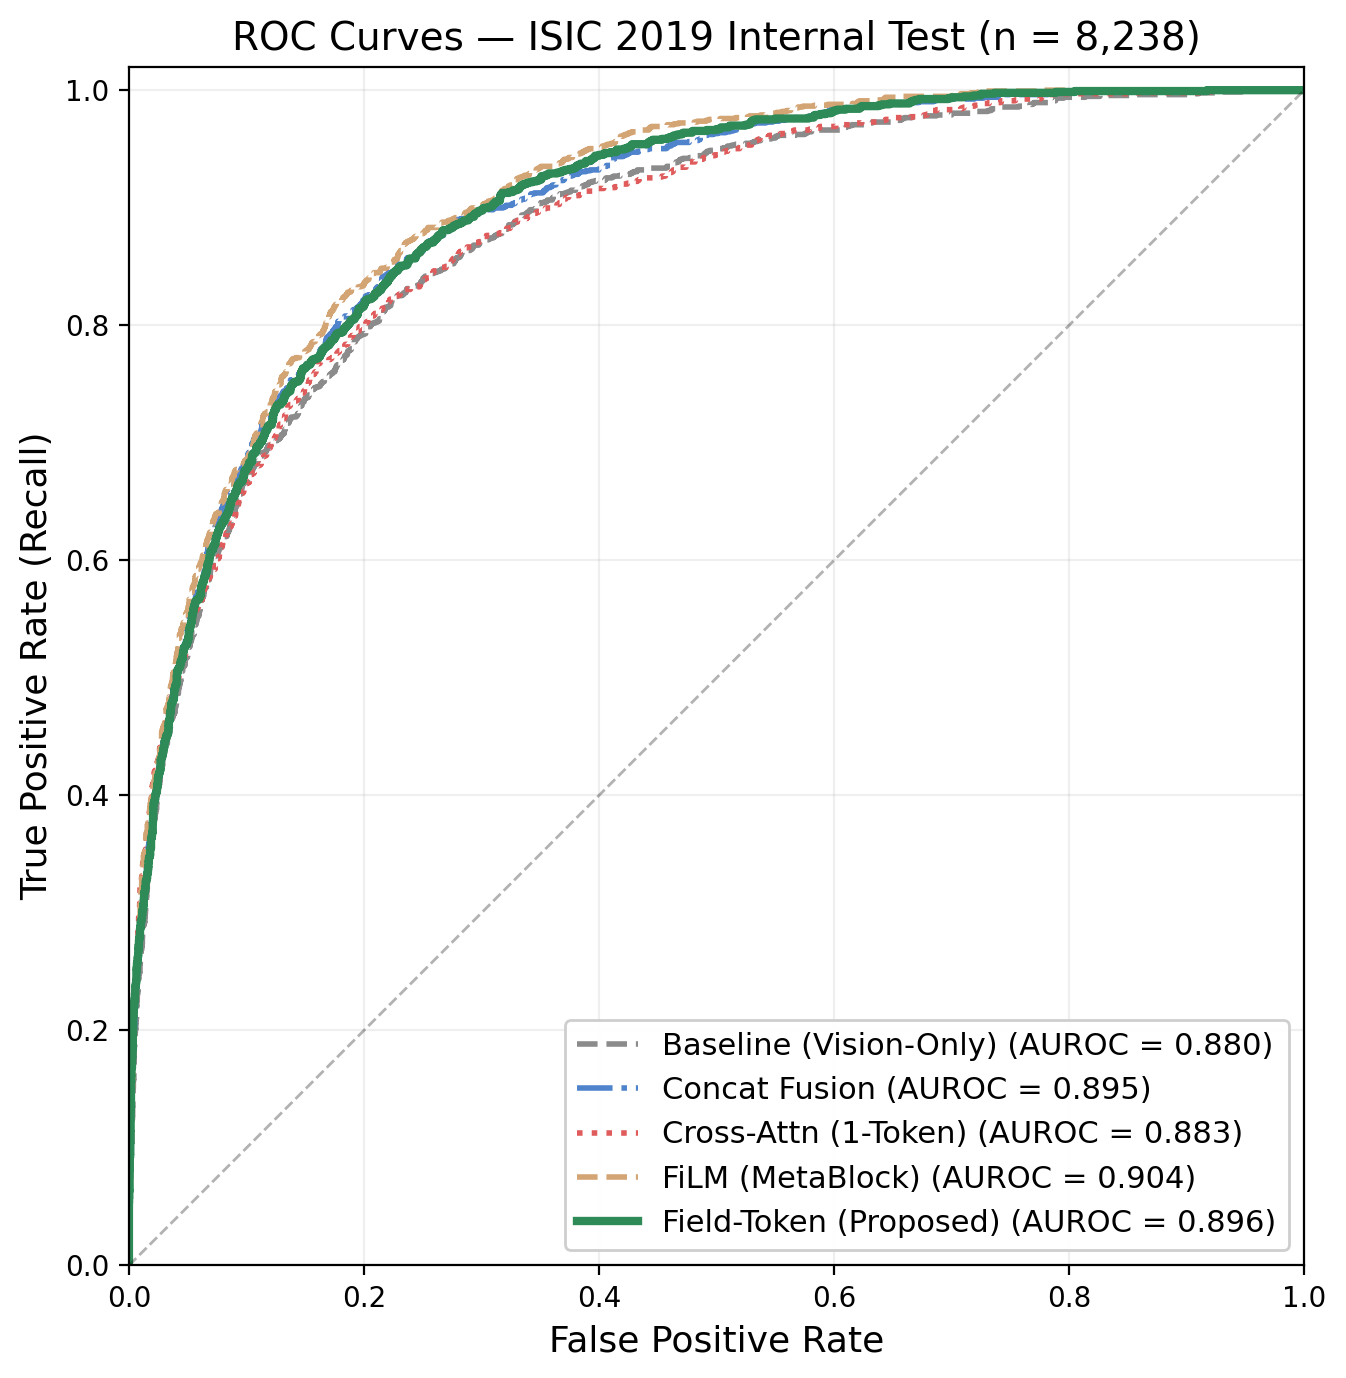
\includegraphics[width=0.85\textwidth]{figures/roc_curves.png}
    \caption{Receiver operating characteristic (ROC) curves for all five models on the ISIC 2019 internal test set ($n = 8{,}238$). Field-Token (proposed, solid green) achieves AUROC = 0.896, second only to FiLM (0.904). The proposed method's curve lies distinctly above the vision-only baseline, particularly in the clinically relevant high-sensitivity region (TPR $> 0.8$).}
    \label{fig:roc}
\end{figure}

\subsection{Extended Evaluation Metrics}

\Cref{tab:extended_metrics} reports AUPRC with 95\% bootstrap CIs, sensitivity at prespecified specificity levels, and Brier scores. FiLM achieves the highest AUPRC (0.690) and highest sensitivity at both the 90\% and 95\% specificity operating points. At 95\% specificity, FiLM retains 55.7\% sensitivity compared with 51.8\% for the baseline---a modest but consistent advantage. Field-Token achieves the second-highest specificity at 90\% sensitivity (0.695), consistent with its higher threshold-dependent recall profile.

\begin{table}[htbp]
\centering
\caption{Extended evaluation metrics on the ISIC 2019 test set (8{,}238 images). AUPRC: area under the precision--recall curve with 95\% percentile bootstrap CIs (1{,}000 iterations, image-level). Sensitivity at prespecified specificity levels of 90\% and 95\%.}
\label{tab:extended_metrics}
\footnotesize
\begin{tabular}{lccccc}
\toprule
Model & AUPRC [95\% CI] & Sens@Spec$\geq$90\% & Sens@Spec$\geq$95\% & Spec@Sens$\geq$90\% & Brier \\
\midrule
Baseline & 0.650 [0.622--0.677] & 0.667 & 0.518 & 0.654 & 0.154 \\
Concat & 0.679 [0.654--0.704] & 0.684 & 0.543 & 0.682 & 0.184 \\
Cross-Attn & 0.671 [0.647--0.696] & 0.665 & 0.528 & 0.640 & 0.144 \\
Field-Token$^\dagger$ & 0.679 [0.653--0.703] & 0.677 & 0.531 & 0.695 & 0.148 \\
FiLM & \textbf{0.690} [0.666--0.715] & \textbf{0.686} & \textbf{0.557} & \textbf{0.705} & 0.150 \\
\bottomrule
\end{tabular}
\end{table}

\subsection{Cross-Dataset Evaluation (ISIC 2020)}

\Cref{tab:external} presents the cross-dataset evaluation results. A striking pattern emerges: models with more expressive metadata conditioning (FiLM, field-token) exhibit larger relative AUROC drops (15.5\% and 16.7\%, respectively), while simpler fusion strategies (concatenation, single-token) degrade less (11.1\% and 10.0\%). This suggests that expressive metadata conditioning risks overfitting to dataset-specific covariate distributions---ISIC 2019 and 2020 differ in patient demographics, imaging protocols, and class balance. Notably, field-token retains the highest cross-dataset recall (0.579), maintaining its advantage in melanoma detection.

\begin{table}[htbp]
\centering
\caption{Cross-dataset evaluation on ISIC 2020 ($n = 33{,}126$, 1.8\% melanoma). $\Delta$AUROC: relative drop from internal test.}
\label{tab:external}
\begin{tabular}{lcccc}
\toprule
Model & AUROC & 95\% CI & Recall & $\Delta$AUROC \\
\midrule
Concat & \textbf{0.796} & [0.776--0.817] & 0.469 & $-$11.1\% \\
Cross-Attn & 0.795 & [0.777--0.815] & 0.462 & $-$10.0\% \\
FiLM & 0.764 & [0.742--0.787] & 0.538 & $-$15.5\% \\
Baseline & 0.763 & [0.742--0.785] & 0.541 & $-$13.3\% \\
Field-Token$^\dagger$ & 0.746 & [0.724--0.769] & \textbf{0.579} & $-$16.7\% \\
\bottomrule
\end{tabular}
\end{table}

\Cref{fig:generalization} visualises this conditioning--generalisation trade-off, highlighting the inverse relationship between conditioning expressiveness and cross-dataset robustness.

\begin{figure}[htbp]
    \centering
    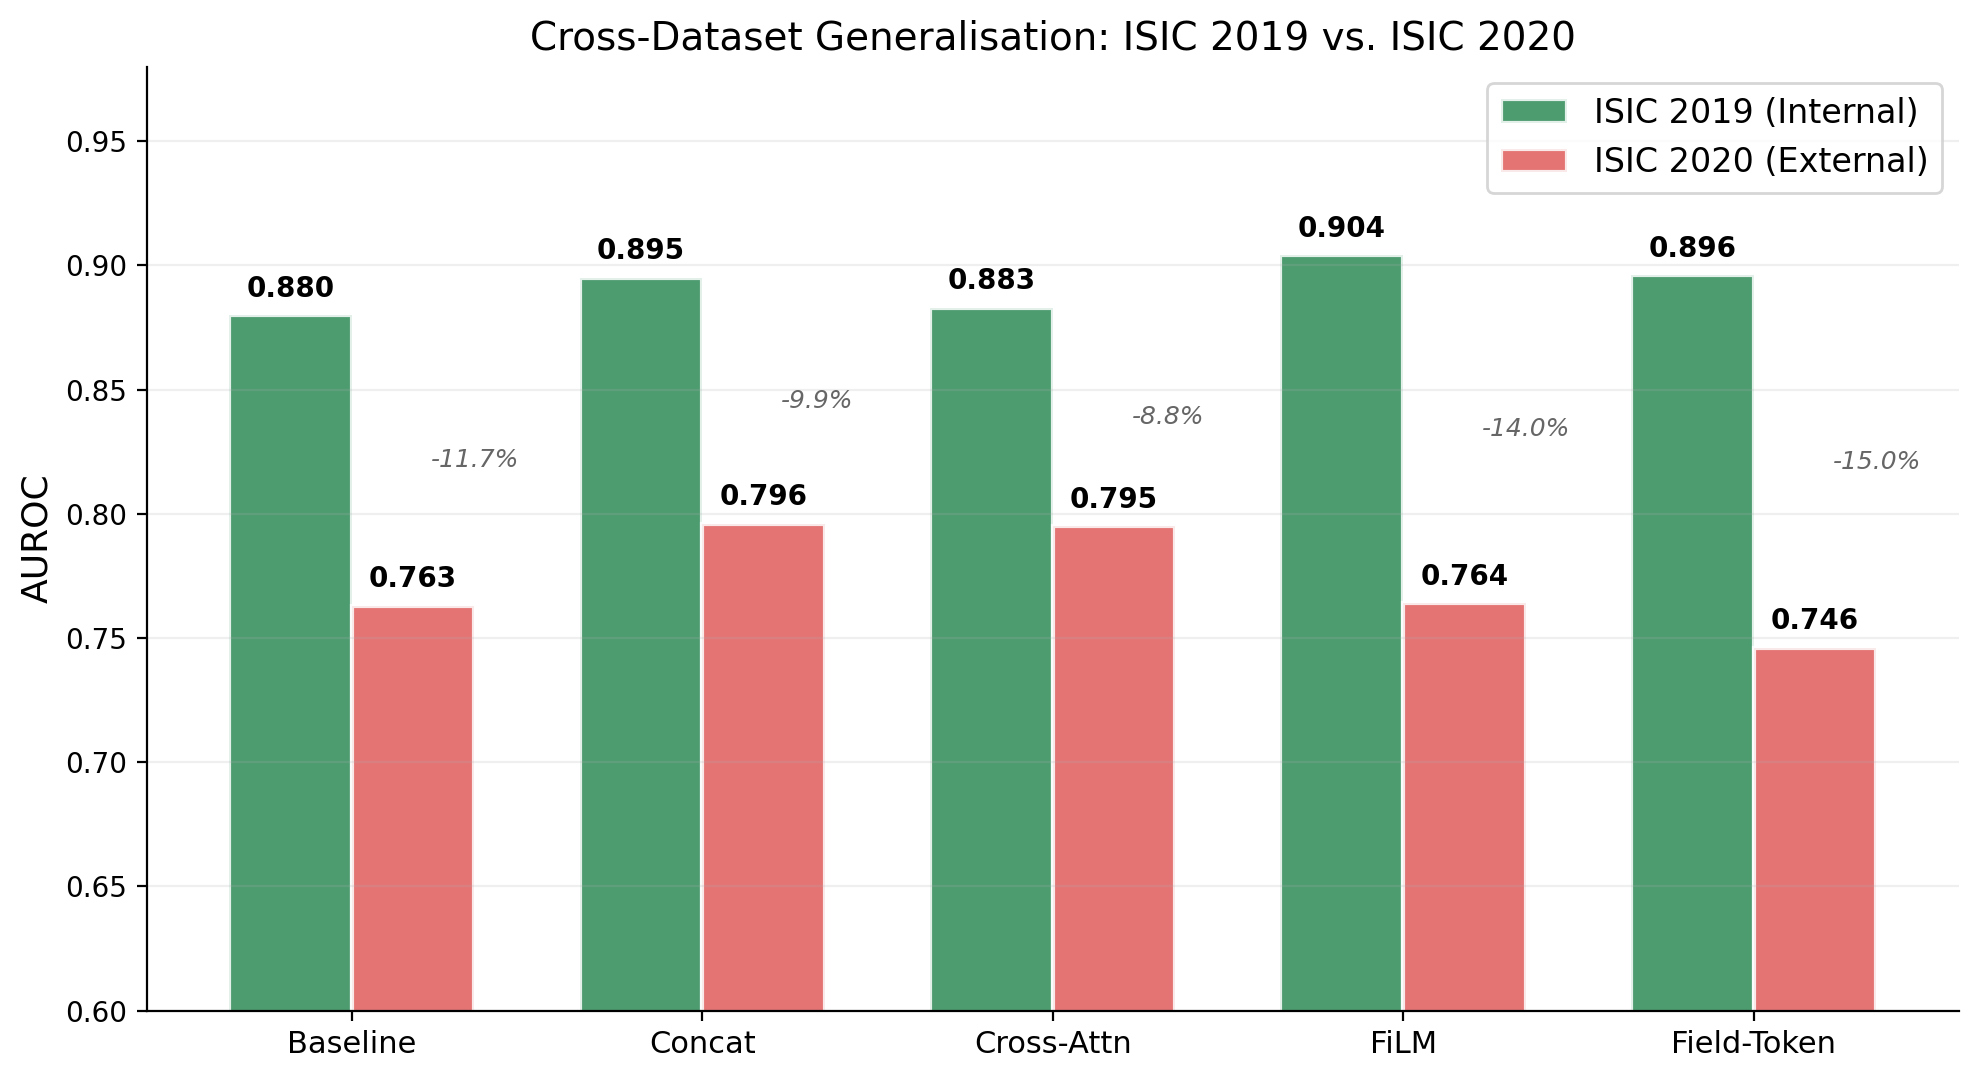
\includegraphics[width=0.9\textwidth]{figures/internal_vs_external.png}
    \caption{Cross-dataset generalisation comparison. Green bars show ISIC 2019 internal AUROC; red bars show ISIC 2020 cross-dataset AUROC. Percentage annotations indicate relative AUROC drop. More expressive conditioning (FiLM, Field-Token) achieves higher internal performance but suffers larger relative drops ($-15.5\%$ to $-16.7\%$) compared to simpler methods ($-10.0\%$ to $-11.1\%$). The baseline drops $-13.3\%$.}
    \label{fig:generalization}
\end{figure}

\subsection{Statistical Significance}

\Cref{tab:delong} reports DeLong pairwise tests on the ISIC 2019 test set with Holm--Bonferroni correction for 10 comparisons. All metadata-augmented models (except single-token cross-attention) significantly outperform the vision-only baseline after multiplicity correction ($p_{\text{Holm}} < 0.001$ for all three). FiLM significantly outperforms field-token ($p_{\text{Holm}} = 0.016$), though with lower recall. Field-token significantly outperforms both the baseline ($p_{\text{Holm}} < 0.001$) and single-token cross-attention ($p_{\text{Holm}} < 0.001$). The Concat--FiLM ($p_{\text{Holm}} = 0.011$) and Field-Token--FiLM ($p_{\text{Holm}} = 0.016$) comparisons are significant at the 0.05 but not the 0.01 level. These are exploratory pairwise comparisons, not preregistered hypotheses.

\begin{table}[htbp]
\centering
\caption{DeLong pairwise AUROC comparisons on ISIC 2019 test set with Holm--Bonferroni correction for 10 comparisons. $^{***}p_{\text{Holm}} < 0.001$; $^{*}p_{\text{Holm}} < 0.05$; ns: not significant.}
\label{tab:delong}
\footnotesize
\begin{tabular}{llcccc}
\toprule
Model A & Model B & $z$ & $p$-raw & $p_{\text{Holm}}$ & Sig. \\
\midrule
Baseline & FiLM & $-$6.57 & $<$0.001 & $<$0.001 & *** \\
Baseline & Field-Token & $-$4.34 & $<$0.001 & $<$0.001 & *** \\
Baseline & Concat & $-$4.69 & $<$0.001 & $<$0.001 & *** \\
Baseline & Cross-Attn & $-$0.65 & 0.514 & 1.000 & ns \\
Cross-Attn & FiLM & $-$6.34 & $<$0.001 & $<$0.001 & *** \\
Cross-Attn & Field-Token & $-$3.92 & $<$0.001 & $<$0.001 & *** \\
Concat & Cross-Attn & $+$3.74 & $<$0.001 & $<$0.001 & *** \\
Concat & FiLM & $-$2.98 & 0.003 & 0.011 & * \\
Concat & Field-Token & $-$0.18 & 0.856 & 1.000 & ns \\
Field-Token & FiLM & $-$2.79 & 0.005 & 0.016 & * \\
\bottomrule
\end{tabular}
\end{table}

\subsection{Calibration Analysis}

All models exhibit overconfidence (learned temperature $T > 1$; \Cref{tab:calibration}), consistent with findings in the broader literature on neural network calibration~\citep{guo2017calibration}. Single-token cross-attention achieves the best raw calibration (ECE = 0.133), while FiLM and field-token have moderate ECE values (0.203, 0.186) despite strong discrimination. Post-hoc temperature scaling improves Brier scores across all models, and we recommend its application in any deployment pipeline. \Cref{fig:reliability} confirms that all models lie below the diagonal, indicating systematic overconfidence.

\begin{table}[htbp]
\centering
\caption{Calibration metrics and temperature scaling results.}
\label{tab:calibration}
\begin{tabular}{lcccc}
\toprule
Model & ECE $\downarrow$ & Brier $\downarrow$ & Temp.\ $T$ & Brier (scaled) $\downarrow$ \\
\midrule
Cross-Attn & \textbf{0.133} & \textbf{0.144} & 2.13 & \textbf{0.137} \\
Baseline & 0.164 & 0.154 & 1.98 & 0.142 \\
Field-Token$^\dagger$ & 0.186 & 0.148 & 1.53 & 0.145 \\
FiLM & 0.203 & 0.150 & 1.45 & 0.148 \\
Concat & 0.237 & 0.184 & 2.05 & 0.171 \\
\bottomrule
\end{tabular}
\end{table}

\begin{figure}[htbp]
    \centering
    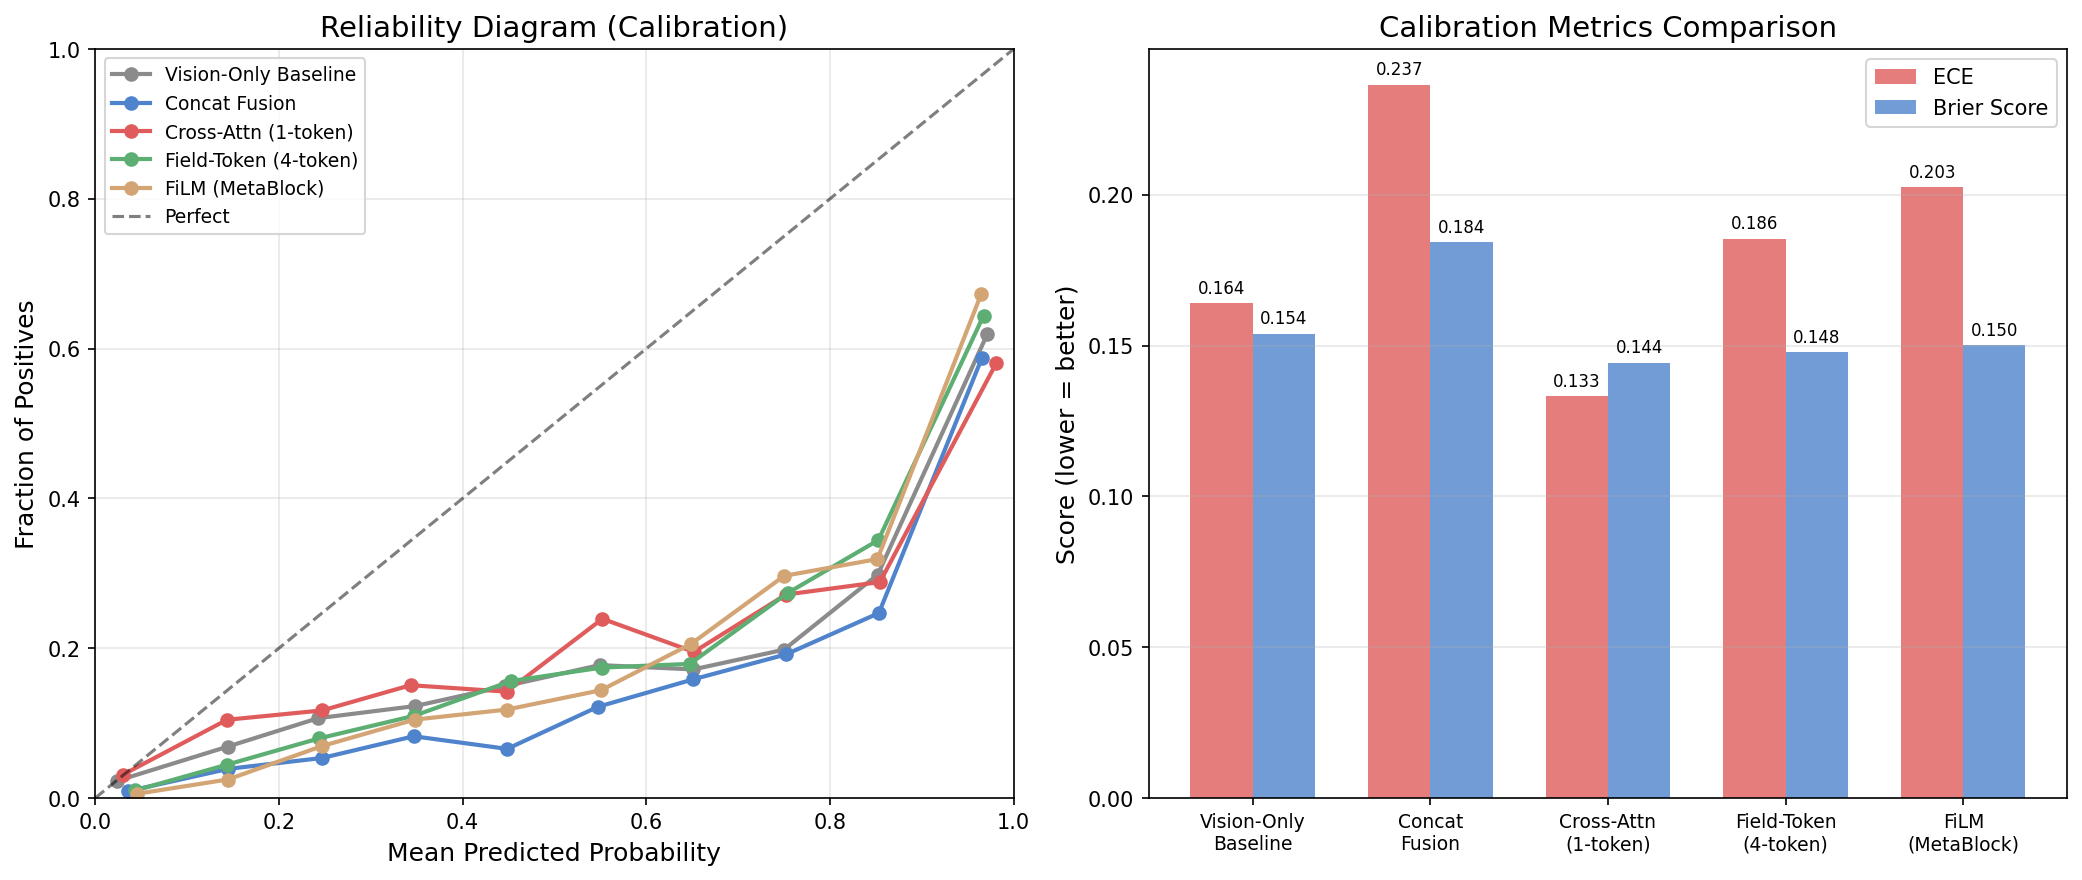
\includegraphics[width=\textwidth]{figures/reliability_diagrams.png}
    \caption{Reliability diagrams and calibration metrics for all five models on ISIC 2019 test set. All models lie below the diagonal, indicating systematic overconfidence.}
    \label{fig:reliability}
\end{figure}

\subsection{Training Robustness}

To assess sensitivity to random initialisation, we retrained all five architectures plus a parameter-matched control across five random seeds (42, 123, 456, 789, 2024). \Cref{tab:multi_seed} reports mean $\pm$ standard deviation on the ISIC~2019 test set. All models show low AUROC variance ($\sigma \leq 0.008$), confirming that the single-seed results reported in the primary analysis are representative. FiLM achieves the highest mean AUROC (0.892$\pm$0.008), followed by Concat (0.892$\pm$0.004) and Field-Token (0.889$\pm$0.007), with overlapping confidence intervals.

\begin{table}[htbp]
\centering
\caption{Multi-seed evaluation on ISIC 2019 test set ($n = 5$ seeds: 42, 123, 456, 789, 2024). Results are reported as mean $\pm$ standard deviation. Threshold-dependent metrics use the Youden-optimal threshold from each seed's validation set. Baseline-Wide is a parameter-matched image-only control (9.02M parameters, widened MLP classifier).}
\label{tab:multi_seed}
\resizebox{\textwidth}{!}{%
\begin{tabular}{lcccccc}
\toprule
Model & AUROC & AUPRC & Recall & Specificity & F1 & Brier \\
\midrule
Baseline (7.88M) & 0.882$\pm$0.002 & 0.634$\pm$0.013 & 0.791$\pm$0.012 & 0.802$\pm$0.013 & 0.560$\pm$0.009 & 0.181$\pm$0.027 \\
Baseline-Wide (9.02M) & 0.876$\pm$0.002 & 0.622$\pm$0.009 & 0.776$\pm$0.024 & 0.807$\pm$0.016 & 0.558$\pm$0.006 & 0.139$\pm$0.015 \\
Concat & 0.892$\pm$0.004 & 0.665$\pm$0.011 & 0.796$\pm$0.049 & 0.811$\pm$0.044 & 0.575$\pm$0.025 & 0.165$\pm$0.015 \\
Cross-Attn & 0.885$\pm$0.004 & 0.650$\pm$0.012 & 0.779$\pm$0.024 & 0.817$\pm$0.025 & 0.571$\pm$0.015 & 0.154$\pm$0.019 \\
Field-Token$^\dagger$ & 0.889$\pm$0.007 & 0.655$\pm$0.018 & 0.792$\pm$0.038 & 0.818$\pm$0.038 & 0.580$\pm$0.022 & 0.164$\pm$0.029 \\
FiLM & 0.892$\pm$0.008 & 0.661$\pm$0.021 & 0.816$\pm$0.024 & 0.798$\pm$0.030 & 0.570$\pm$0.021 & 0.145$\pm$0.012 \\
\bottomrule
\end{tabular}%
}
\end{table}

\textbf{Parameter-matched control.} The Baseline-Wide model uses the same EfficientNet-B2 backbone as all other models but replaces the narrow classification head with a widened MLP (9.02M total parameters, exceeding Field-Token's 8.96M). Despite having more parameters than any other model, Baseline-Wide achieves \emph{lower} AUROC (0.876$\pm$0.002) than even the original Baseline (0.882$\pm$0.002), suggesting that additional MLP capacity without structured metadata integration does not improve discrimination and may lead to overfitting. Field-Token's improvement over Baseline-Wide ($\Delta = +0.013$) therefore cannot be attributed to parameter count alone.

Pairwise bootstrap analysis (10{,}000 resamples) of the five-seed AUROC distributions confirms that the 95\% confidence interval for the Field-Token--Baseline difference excludes zero ($\Delta = +0.006$, CI $[+0.002, +0.011]$), supporting Field-Token's improvement over the image-only baseline. In contrast, the FiLM--Field-Token difference ($\Delta = +0.003$, CI $[-0.003, +0.009]$) and Concat--Field-Token difference ($\Delta = +0.004$, CI $[+0.000, +0.009]$) both include or border zero, indicating that the top three metadata-conditioning methods are statistically indistinguishable in discrimination. With $n = 5$ seeds, the Wilcoxon signed-rank test has a minimum attainable $p$-value of 0.0625, providing insufficient power for formal significance testing; the bootstrap CIs are therefore more informative.

\subsection{Token-Count Ablation}

To assess whether splitting metadata into four separate tokens is necessary, we trained ablated variants with $K \in \{1, 2, 3\}$ metadata tokens across five seeds, keeping the cross-attention architecture and classifier identical (\Cref{tab:token_ablation}). All variants have nearly identical parameter counts (8.90M--8.96M). \textbf{Note:} these $K$-ablated variants use the field-token metadata encoder with merged token groupings, not the shared metadata encoder used by the main single-token Cross-Attn model in \Cref{tab:internal}. The two $K{=}1$ configurations therefore differ in encoder architecture, explaining the AUROC difference ($0.891 \pm 0.004$ ablated vs.\ $0.885 \pm 0.004$ main Cross-Attn).

\begin{table}[htbp]
\centering
\caption{Token-count ablation ($n = 5$ seeds). $K$ = number of metadata tokens in cross-attention. All variants share the same backbone, cross-attention module, and classifier but use the field-token encoder with merged groupings, not the shared encoder of the main Cross-Attn model.}
\label{tab:token_ablation}
\small
\begin{tabular}{clcc}
\toprule
$K$ & Token Grouping & AUROC & Per-Variable Routing \\
\midrule
1 & [all metadata merged] & 0.891$\pm$0.004 & None \\
2 & [demographic, site] & 0.888$\pm$0.007 & Partial \\
3 & [age{+}miss, sex, site] & 0.887$\pm$0.002 & Partial \\
4 & [age, sex, site, miss] & 0.889$\pm$0.007 & Full \\
\bottomrule
\end{tabular}
\end{table}

\Cref{fig:token_ablation} visualises the AUROC plateau across token counts, with the baseline reference line for comparison.

\begin{figure}[htbp]
    \centering
    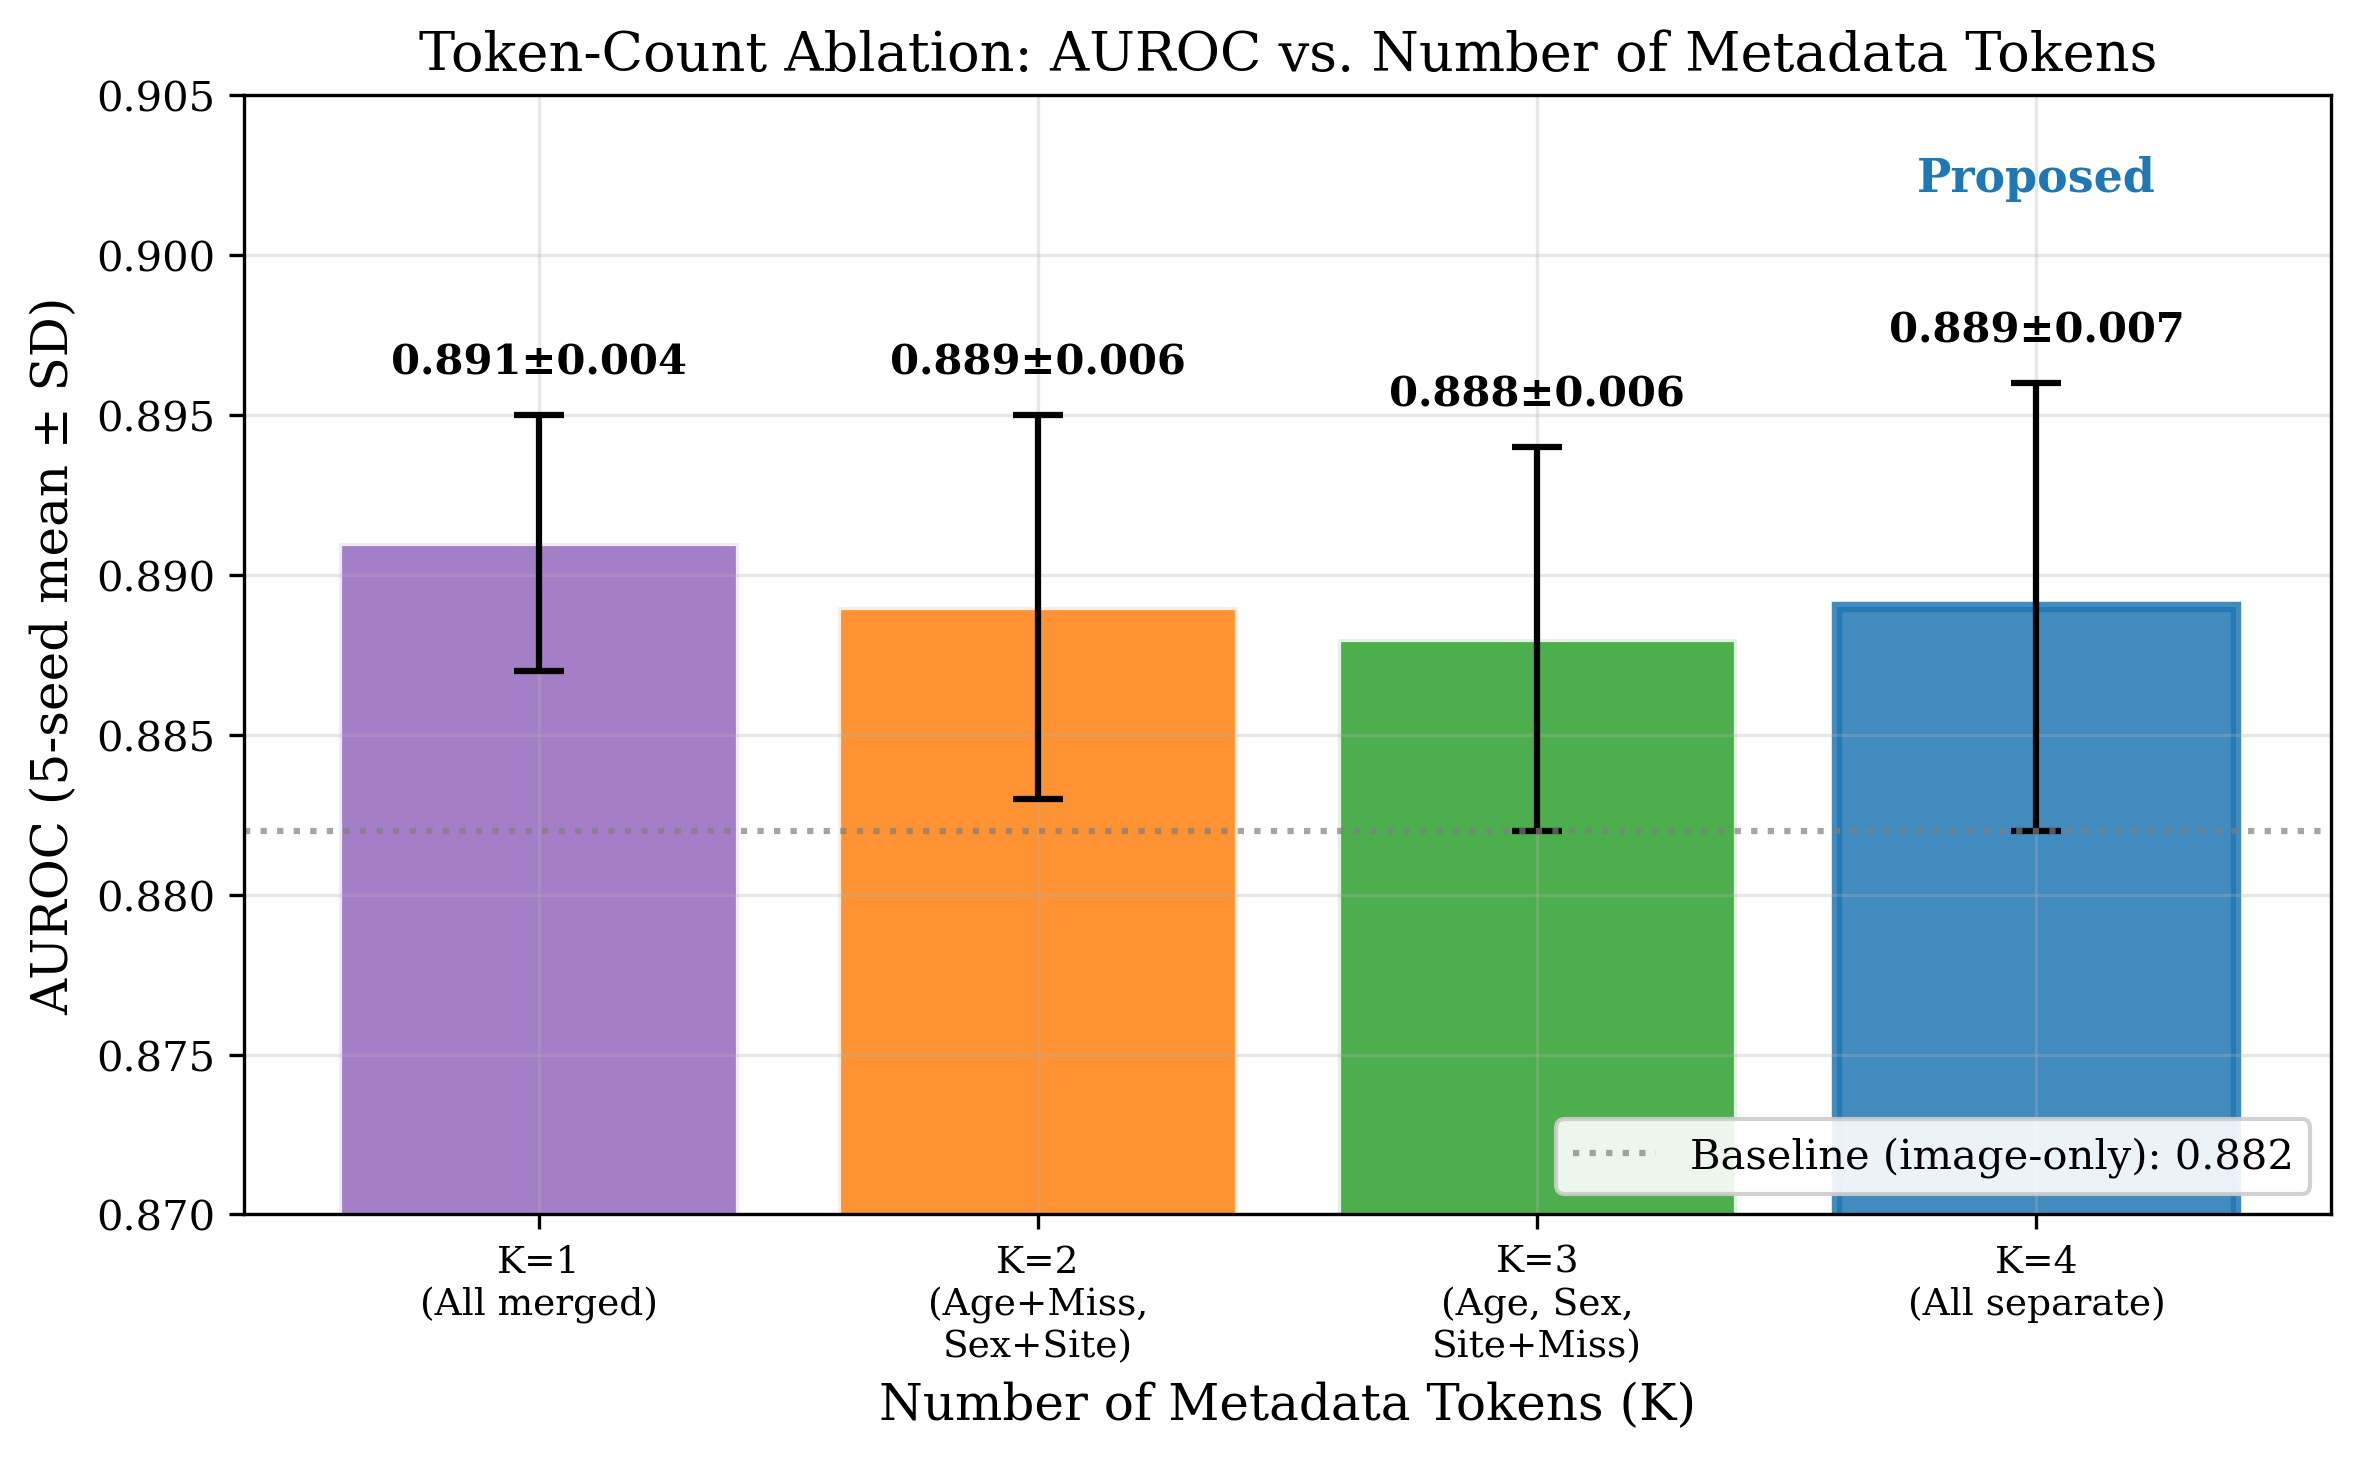
\includegraphics[width=0.85\textwidth]{figures/token_ablation_chart.png}
    \caption{Token-count ablation: AUROC (5-seed mean $\pm$ SD) as a function of the number of metadata tokens $K$. The dashed line marks the image-only baseline (0.882). AUROC is stable across all values of $K$; the proposed $K{=}4$ configuration is selected for its structural interpretability (per-variable routing), not discrimination advantage.}
    \label{fig:token_ablation}
\end{figure}

AUROC is flat across all token counts (range: 0.004), with overlapping bootstrap CIs. The advantage of $K{=}4$ is structural rather than discriminative: it produces field-indexed $49 \times 4$ routing maps and enables the per-variable sensitivity analysis in \Cref{sec:counterfactual}.

\subsection{Image-Fixed Model-Sensitivity Analysis}

The image-fixed intervention protocol was applied to all $n = 1{,}327$ melanoma-positive test cases using the field-token model. These are model-level sensitivity properties---they describe the model's learned input--output relationships, not causal or epidemiological effects. Results are summarised in \Cref{tab:counterfactual}.

\textbf{Age sensitivity.} The mean predicted probability rises from $\bar{p} = 0.564$ (age 10) to $\bar{p} = 0.834$ (age 85), with 94.3\% of cases showing monotonically non-decreasing output. The mean sensitivity of 0.274 (27.4 percentage points) confirms non-trivial modulation, ruling out insensitivity. The steepest rise occurs between ages 25--55, consistent with the epidemiological age--incidence relationship~\citep{whiteman2016growing}.

\textbf{Anatomical site sensitivity.} Site replacement yields the highest outputs for palms/soles (0.866) and upper extremities (0.855), and the lowest for unknown site (0.642), broadly consistent with clinical knowledge of acral melanoma presentation~\citep{bradford2009acral}.

\textbf{Sex sensitivity.} The sex effect is small ($\Delta p = 0.018$): female ($\bar{p} = 0.801$) slightly exceeds male ($\bar{p} = 0.783$).

\begin{table}[htbp]
\centering
\caption{Image-fixed model-sensitivity analysis ($n = 1{,}327$ melanoma cases, field-token model).}
\label{tab:counterfactual}
\begin{tabular}{lcc}
\toprule
Variable & Key Finding & Magnitude \\
\midrule
Age & 94.3\% monotonicity rate & $\Delta p = 0.270$ (age 10$\to$85) \\
Site & palms/soles highest model output & $p_{\max} - p_{\min} = 0.225$ \\
Sex & female slightly higher & $\Delta p = 0.018$ \\
\bottomrule
\end{tabular}
\end{table}

\textbf{Cross-model comparison.} Applying the same protocol to FiLM yields similar aggregate sensitivities: 89.3\% age monotonicity ($\Delta p = 0.244$), small sex effect ($\Delta p = 0.009$), and greater site variation ($\Delta p = 0.298$ vs.\ 0.225). The protocol generalises across architectures; the structural difference---field-token's per-variable routing map vs.\ FiLM's monolithic transformation---is discussed in \Cref{sec:discussion}.

\Cref{fig:counterfactual} presents the population-level sensitivity curves, \Cref{fig:cross_model} provides a direct visual comparison of the field-token and FiLM sensitivity profiles, and \Cref{fig:explanation} shows representative explanation panels combining Grad-CAM spatial attention with model-sensitivity plots.

\begin{figure}[htbp]
    \centering
    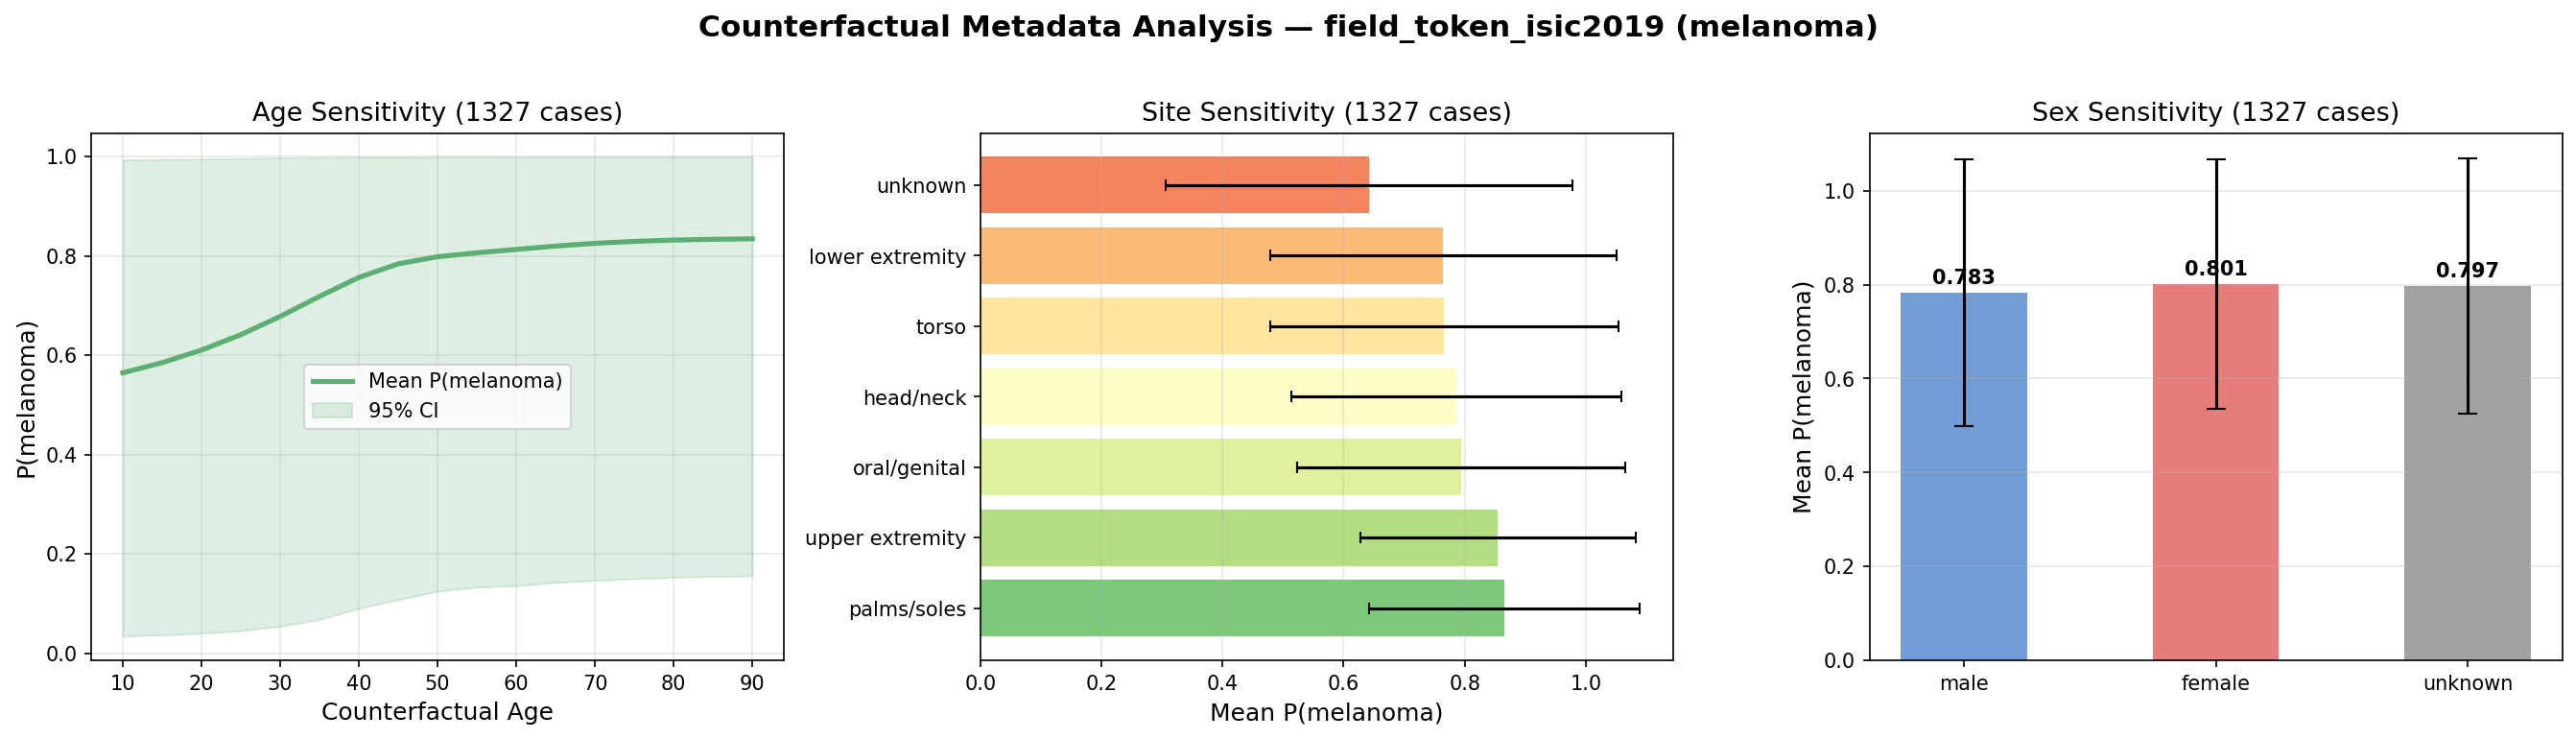
\includegraphics[width=\textwidth]{figures/counterfactual_curves.png}
    \caption{Population-level model-sensitivity curves under synthetic metadata replacement for the field-token model across 1,327 melanoma test cases. (a)~Age sensitivity with pointwise 95\% percentile bootstrap interval ($B=1{,}000$, image-level resampling) for the mean curve. (b)~Anatomical site sensitivity (mean $\pm$ SD). (c)~Sex sensitivity.}
    \label{fig:counterfactual}
\end{figure}

\begin{figure*}[htbp]
    \centering
    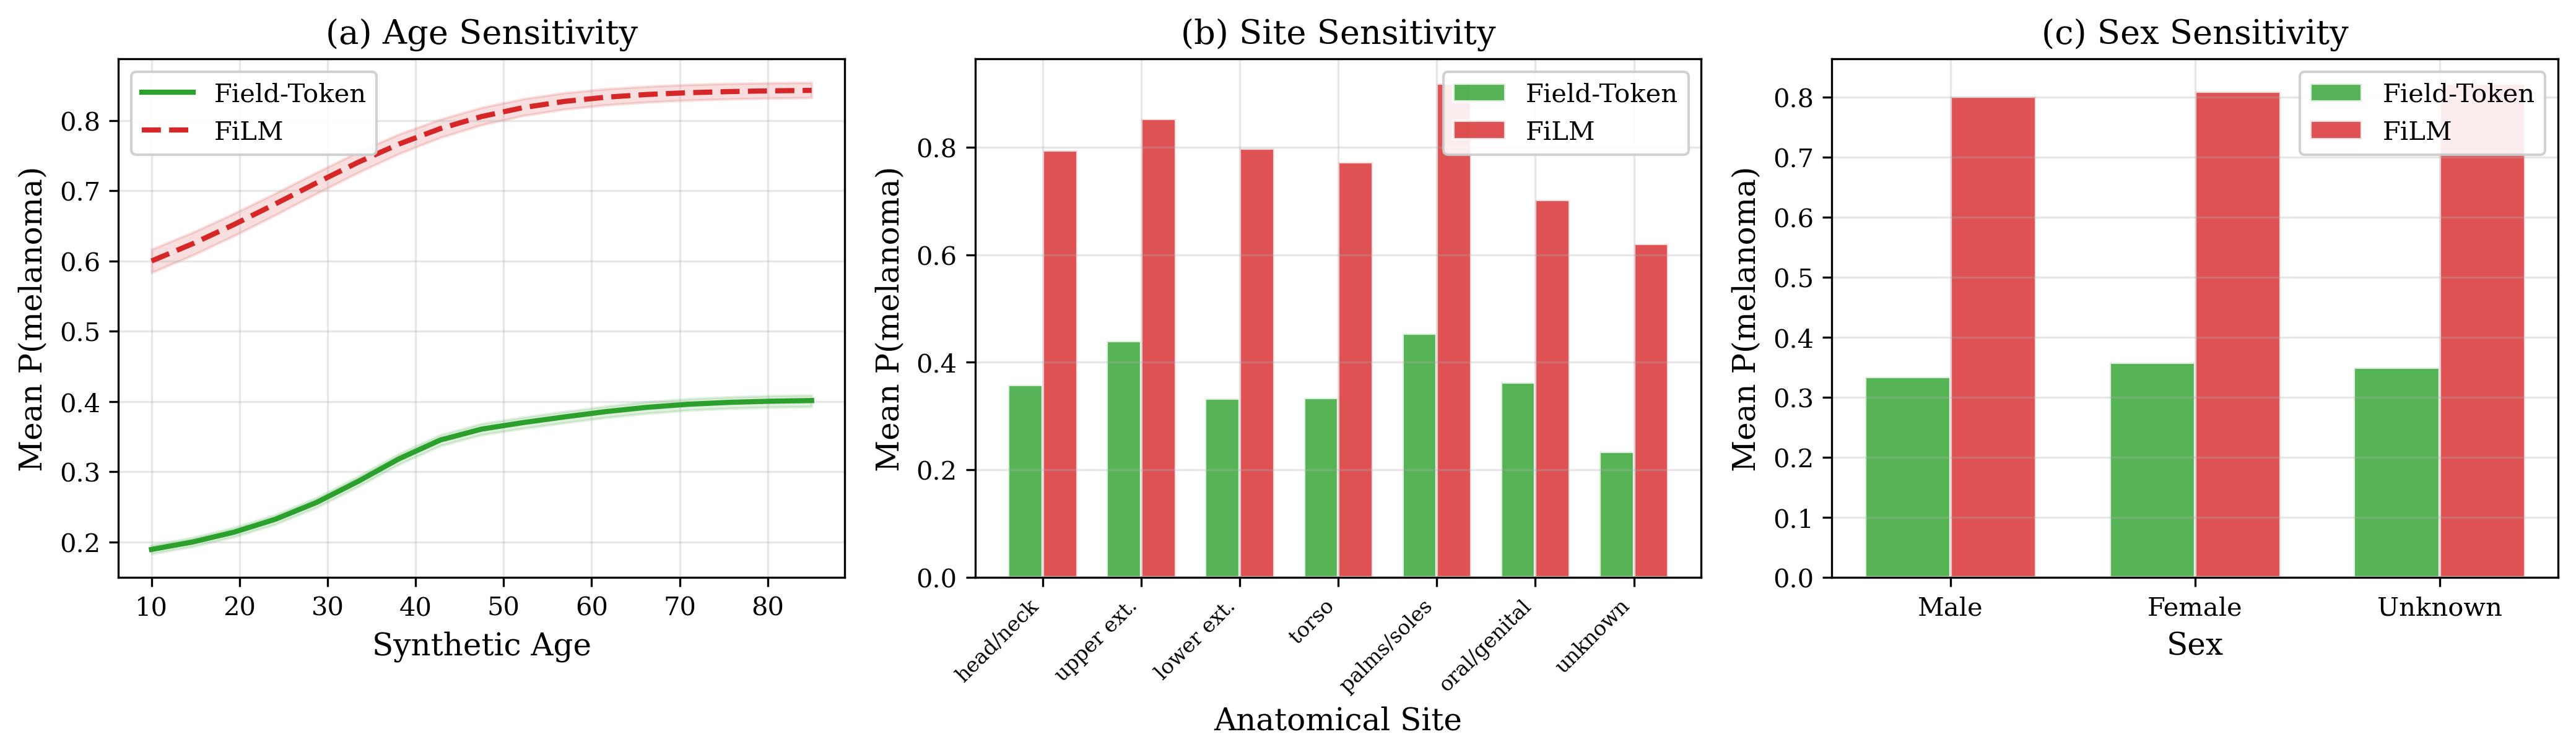
\includegraphics[width=\textwidth]{figures/cross_model_sensitivity.png}
    \caption{Cross-model sensitivity comparison: field-token (green) vs.\ FiLM (red) under the same image-fixed intervention protocol. (a)~Age sensitivity with 95\% bootstrap CI---both models show monotonically increasing melanoma probability with age, but FiLM operates at a higher baseline output. (b)~Anatomical site sensitivity---FiLM exhibits greater inter-site variation ($\Delta p = 0.298$ vs.\ 0.225). (c)~Sex sensitivity---both models show minimal sex-related variation.}
    \label{fig:cross_model}
\end{figure*}


\begin{figure}[htbp]
    \centering
    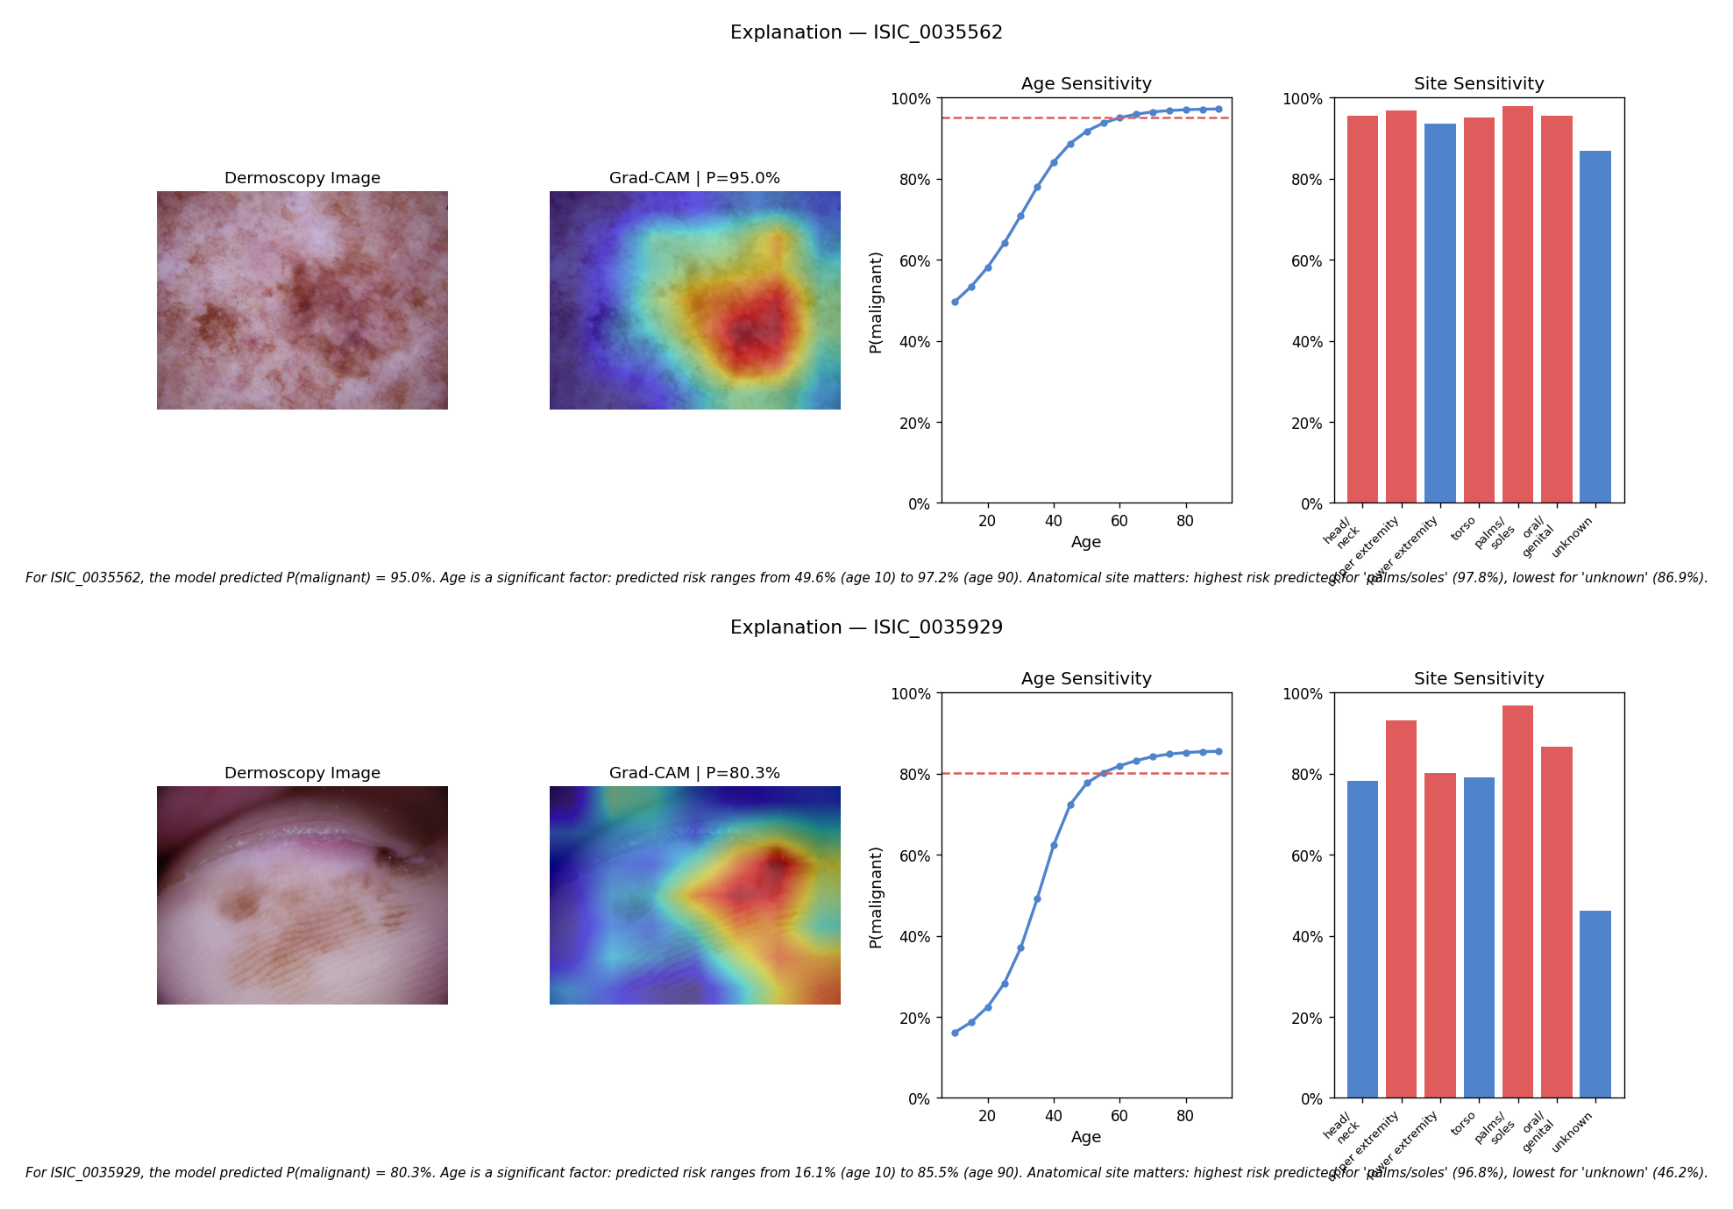
\includegraphics[width=\textwidth]{figures/explanation_panel.png}
    \caption{Example explanation panel for a melanoma case: (a)~original dermoscopic image, (b)~Grad-CAM attention overlay, (c)~age sensitivity curve, (d)~anatomical site sensitivity.}
    \label{fig:explanation}
\end{figure}

\begin{figure*}[htbp]
    \centering
    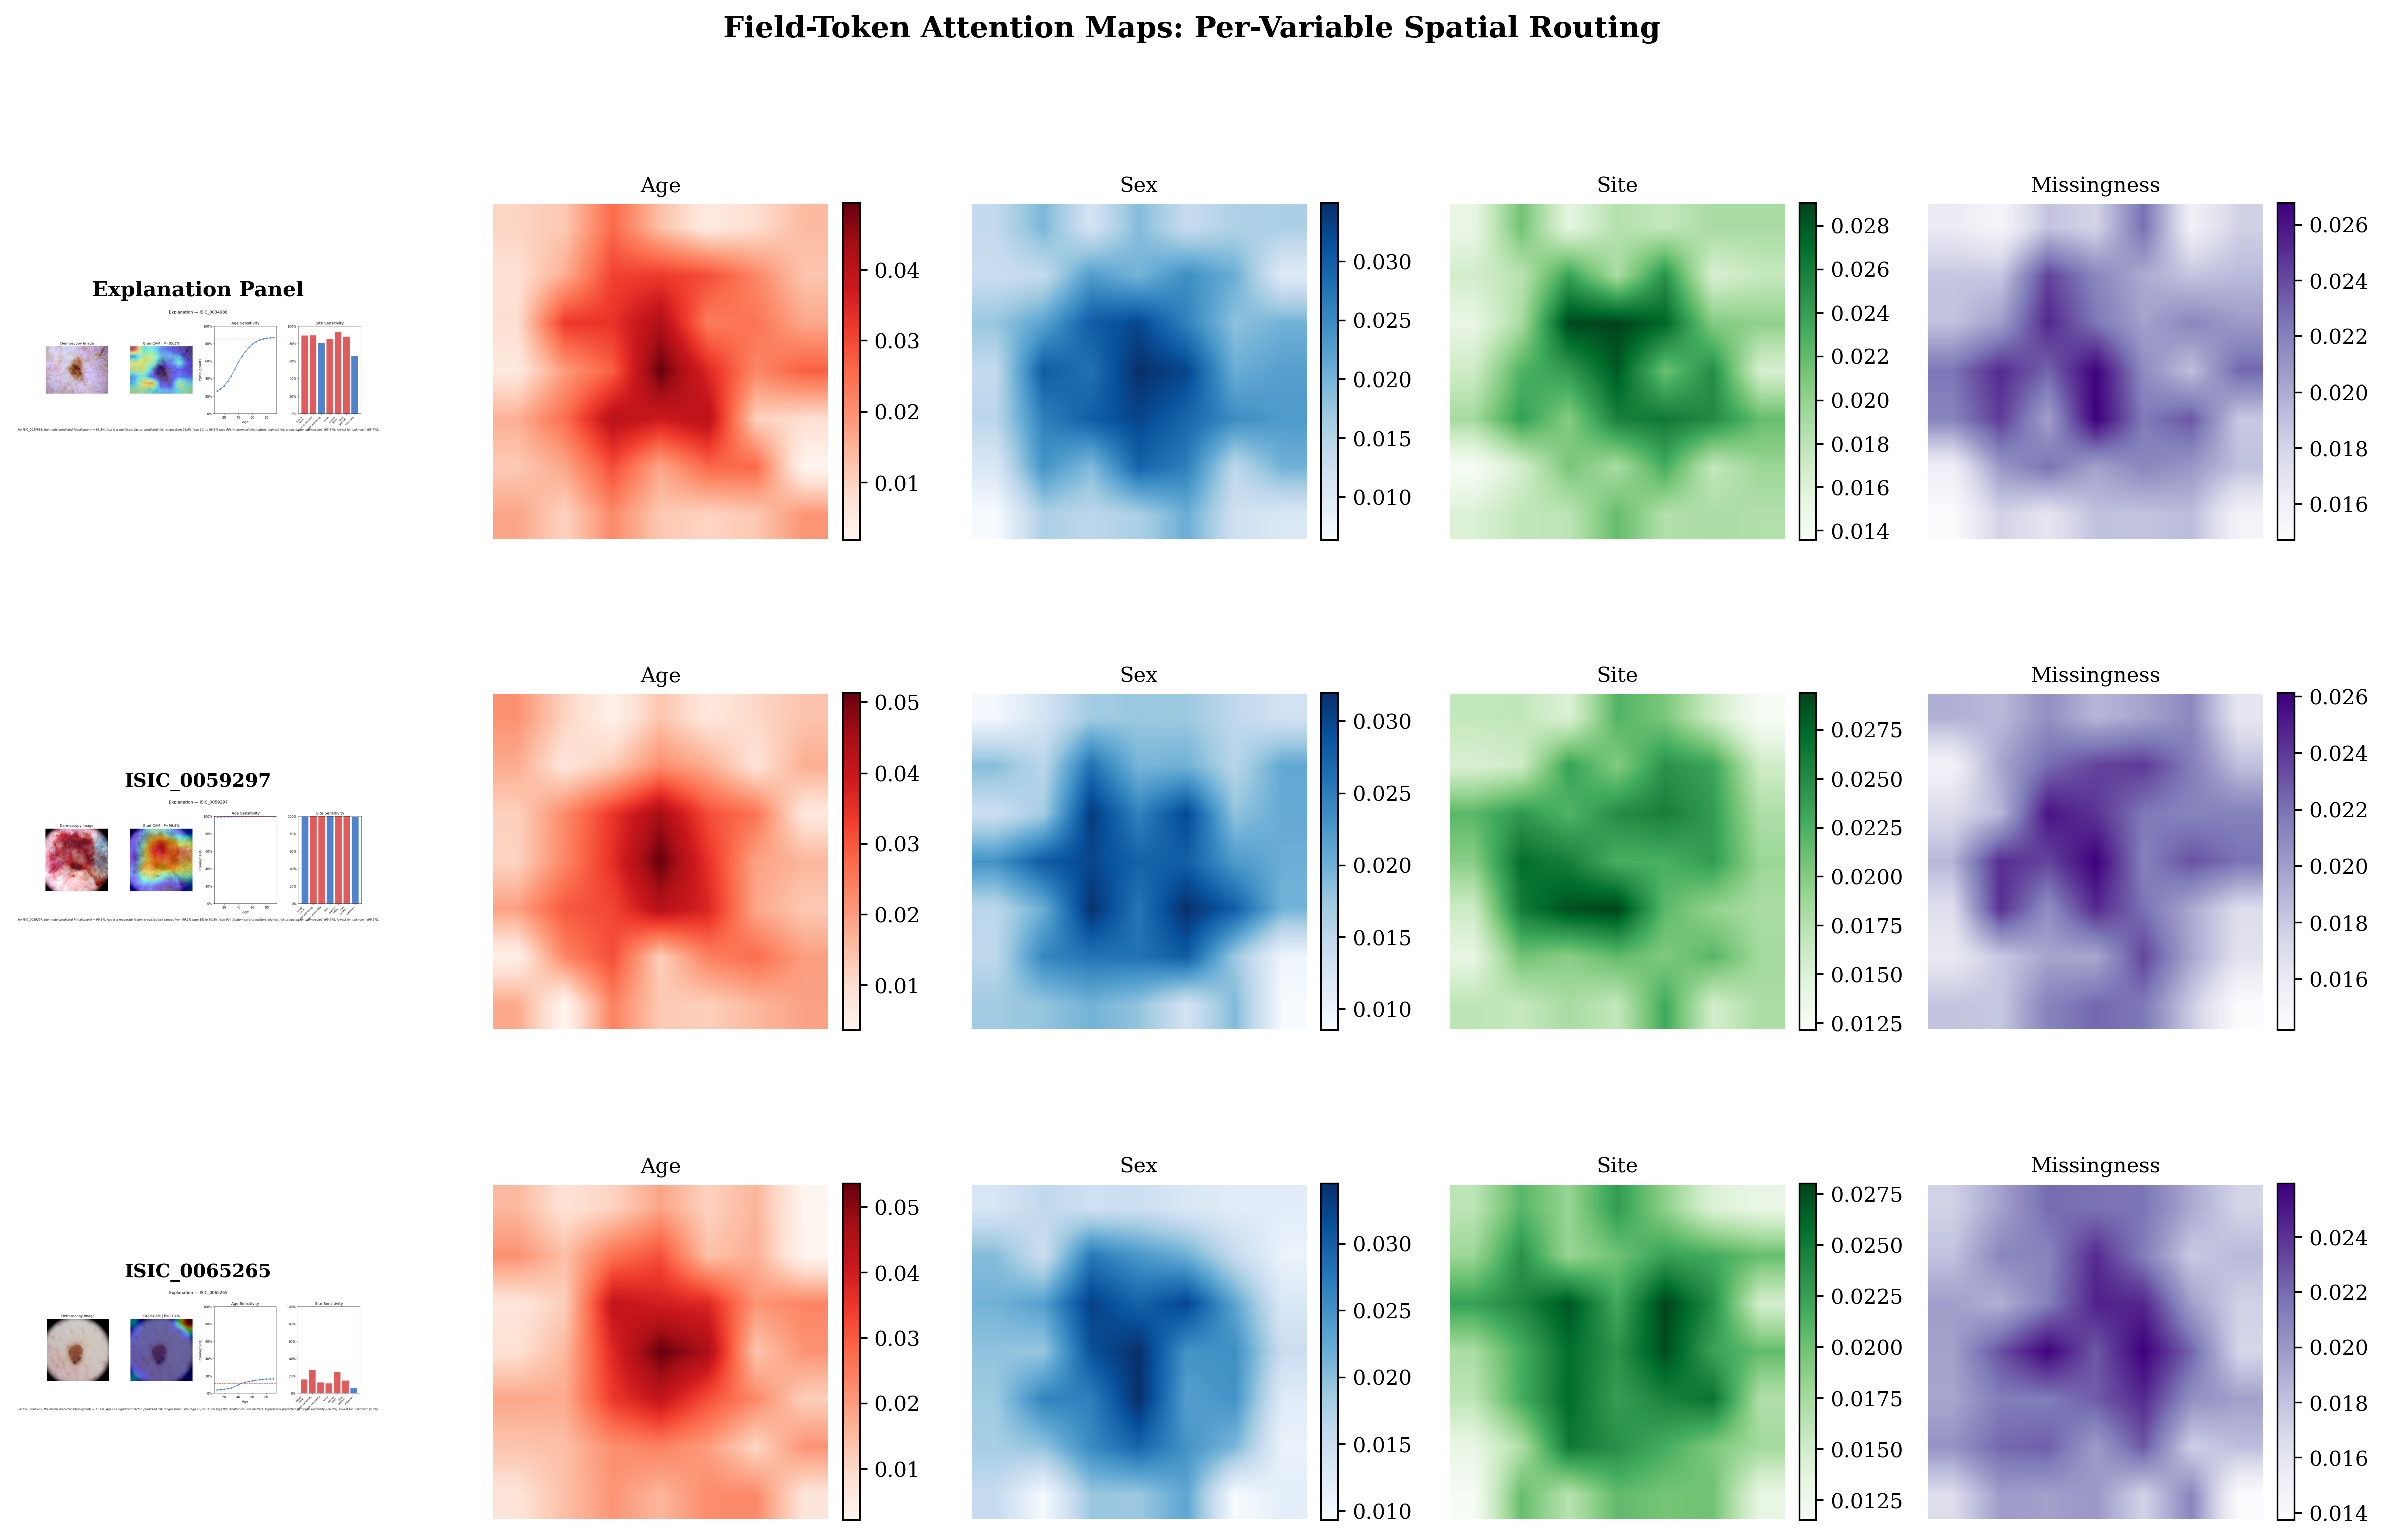
\includegraphics[width=\textwidth]{figures/attention_heatmaps.png}
    \caption{Field-token attention maps for three melanoma cases. Left column: full explanation panel (dermoscopic image, Grad-CAM overlay, sensitivity curves). Right four columns: per-variable spatial attention weights ($7 \times 7$) for age, sex, site, and missingness tokens. Each metadata field routes attention to different spatial regions, enabling per-variable interpretability---a structural property unique to the field-token architecture.}
    \label{fig:attention_heatmaps}
\end{figure*}

% ============================================================
% 7. DISCUSSION
% ============================================================
\section{Discussion}
\label{sec:discussion}

\subsection{Field-Token vs.\ FiLM: Structured Conditioning vs.\ Performance}

FiLM and field-token are functionally equivalent in discrimination: FiLM leads on seed 42 (0.904 vs.\ 0.896, $p = 0.005$), but across five seeds the gap is not significant ($\Delta = 0.003$, CI $[-0.003, +0.009]$). The practical difference is structural. FiLM applies a monolithic affine transformation; field-token produces a $49 \times 4$ routing map (\Cref{eq:attention_weights}) that shows which spatial positions attend to which metadata field---a decomposition FiLM cannot provide. A parameter-matched image-only control (Baseline-Wide, 9.02M parameters) scores \emph{lower} than the original Baseline (0.876 vs.\ 0.882; \Cref{tab:multi_seed}), confirming that simply adding parameters without structured metadata integration does not help. The token-count ablation (\Cref{tab:token_ablation}) shows flat AUROC across $K{=}1{\ldots}4$; $K{=}4$ is chosen for its per-variable decomposition, not for discrimination.

\subsection{The Metadata Conditioning--Generalisation Trade-off}

A consistent pattern emerges across all metadata-conditioning approaches: more expressive conditioning was associated with higher in-distribution performance but larger cross-dataset AUROC reduction in this comparison. FiLM and field-token, which modulate spatial features at a fine-grained level, drop 15--17\% AUROC on ISIC~2020, while concatenation and single-token cross-attention drop only 10--11\%. One hypothesis is that expressive conditioning methods may learn dataset-specific correlations between metadata and diagnosis labels---for instance, the age distribution of melanoma patients may differ between ISIC~2019 and ISIC~2020 due to differences in referral patterns and geographic populations. This finding has practical implications: in deployment scenarios where the metadata distribution is expected to shift, simpler fusion strategies or explicit domain adaptation may be preferable.

\subsection{Descriptive Evaluation of Metadata Sensitivity}
\label{sec:sensitivity_discussion}

Age sweeps raised the predicted melanoma probability in 94.3\% of cases (1{,}251/1{,}327), with a mean shift of 27.4 percentage points from age 10 to 85. A constant-output model would trivially achieve 100\% monotonicity, but the large mean sensitivity rules out insensitivity. No monotonicity constraint was imposed---the pattern emerged from the training data. The site-output ranking (palms/soles $>$ upper extremity $>$ head/neck $>$ torso) aligns with known melanoma predilections~\citep{bradford2009acral, elwood1998distribution}, though acral melanomas are rare in ISIC's predominantly fair-skinned populations, and synthetic site replacement can conflict with visible image morphology. Sex has a small effect ($\Delta p = 0.018$).

These are descriptive properties of the trained model---they show that the conditioning has learned directionally plausible relationships, but they cannot exclude confounding and do not constitute clinical validation. Prospective evaluation with clinician participants remains necessary.

\subsection{Calibration Considerations}

All models are overconfident ($T > 1$), with concatenation showing the worst calibration (ECE = 0.237) and single-token cross-attention the best (ECE = 0.133). This is consistent with the broader finding that modern neural networks are poorly calibrated~\citep{guo2017calibration}. All raw and temperature-scaled Brier scores exceed the empirical-prevalence reference ($BS_{\text{ref}} = p(1-p) = 0.135$ at test prevalence 16.1\%), indicating that the models provide useful ranking but poor probability quality; outputs should be interpreted as relative ordering scores rather than calibrated risk estimates. Temperature $T$ was fitted on validation-set logits only by minimising negative log-likelihood and applied (frozen) to test and cross-dataset predictions. All reported recall, precision and F1 values use raw (uncalibrated) scores at the validation-derived Youden threshold. Post-hoc temperature scaling improves Brier scores uniformly but does not address the positive-weight BCE intercept shift.

\subsection{Limitations}

\textbf{Dataset bias.} The available ISIC metadata do not include a validated skin-tone or Fitzpatrick-type annotation for this analysis. Prior work has documented skin-tone-related performance disparities in dermatology AI~\citep{groh2024deep}, motivating skin-tone-stratified external evaluation on datasets such as PAD-UFES-20~\citep{pacheco2020pad} or the Diverse Dermatology Images dataset~\citep{daneshjou2022disparities} as an important future direction.

\textbf{Binary formulation.} We reduce the eight-class ISIC~2019 problem to binary melanoma detection. Extension to multi-class classification would test whether field-token conditioning improves discrimination for rarer diagnostic categories.

\textbf{UNK test cases.} The official ISIC~2019 test set includes 2{,}047 images labelled UNK---a category absent from the training set. These are mapped to the negative class. To assess the sensitivity of our results to this choice, we re-evaluated all five models on the 6{,}191 known-label test cases (UNK excluded). AUROC changes were small ($|\Delta\text{AUROC}| \leq 0.007$ for all models), and the relative model ranking was unchanged: FiLM remained highest (0.904 $\to$ 0.904), followed by Field-Token (0.896 $\to$ 0.895) and Concat (0.895 $\to$ 0.893). AUPRC increased for all models under UNK exclusion due to higher prevalence (21.4\% vs.\ 16.1\%). We report the full 8{,}238-case results as the primary analysis. The complete known-label comparison is shown in \Cref{tab:unk_sensitivity}. Official challenge weights (\texttt{score\_weight}, \texttt{validation\_weight}) were not used; all image-level evaluations are unweighted.

\begin{table*}[htbp]
\centering
\caption{UNK sensitivity analysis on the ISIC 2019 test set. \textit{All cases}: 8{,}238 images (2{,}047 UNK mapped to negative, prevalence 16.1\%). \textit{Known-label}: 6{,}191 images with confirmed diagnoses (prevalence 21.4\%). The same validation-derived thresholds are applied in both conditions. AUROC CIs are 95\% percentile bootstrap (1{,}000 iterations, image-level).}
\label{tab:unk_sensitivity}
\resizebox{\textwidth}{!}{%
\begin{tabular}{llccccccc}
\toprule
Condition & Model & AUROC [95\% CI] & AUPRC & Recall & Spec & F1 & Brier & $\Delta$AUROC \\
\midrule
All ($n$=8{,}238) & Baseline & 0.880 [0.870--0.890] & 0.650 & 0.802 & 0.791 & 0.554 & 0.154 & --- \\
Known ($n$=6{,}191) & Baseline & 0.879 [0.868--0.890] & 0.729 & 0.802 & 0.783 & 0.617 & 0.156 & $-$0.001 \\
\addlinespace
All ($n$=8{,}238) & Concat & 0.895 [0.886--0.904] & 0.679 & 0.729 & 0.877 & 0.616 & 0.184 & --- \\
Known ($n$=6{,}191) & Concat & 0.893 [0.883--0.902] & 0.743 & 0.729 & 0.875 & 0.667 & 0.184 & $-$0.002 \\
\addlinespace
All ($n$=8{,}238) & Cross-Attn & 0.883 [0.873--0.892] & 0.671 & 0.769 & 0.834 & 0.584 & 0.144 & --- \\
Known ($n$=6{,}191) & Cross-Attn & 0.889 [0.878--0.900] & 0.749 & 0.769 & 0.848 & 0.661 & 0.138 & $+$0.007 \\
\addlinespace
All ($n$=8{,}238) & Field-Token$^\dagger$ & 0.896 [0.887--0.904] & 0.679 & 0.855 & 0.762 & 0.552 & 0.148 & --- \\
Known ($n$=6{,}191) & Field-Token$^\dagger$ & 0.895 [0.886--0.904] & 0.747 & 0.855 & 0.749 & 0.616 & 0.149 & $-$0.001 \\
\addlinespace
All ($n$=8{,}238) & FiLM & 0.904 [0.895--0.912] & 0.690 & 0.796 & 0.835 & 0.599 & 0.150 & --- \\
Known ($n$=6{,}191) & FiLM & 0.904 [0.895--0.912] & 0.762 & 0.796 & 0.832 & 0.660 & 0.149 & $-$0.000 \\
\bottomrule
\end{tabular}%
}
\end{table*}

\textbf{Model-level interventions.} Our sensitivity analysis uses model-level input replacement, not causal interventions. The sensitivity curves reflect learned input--output mappings and should not be interpreted as causal effects of age, sex, or site on melanoma risk.

\textbf{Attention faithfulness.} We empirically tested whether the cross-attention weights are faithful indicators of feature importance by masking the top-9 most-attended spatial positions (18.4\% of 49 total positions, ranked by mean head-averaged attention summed across fields) and replacing them with zeros before the residual addition. We measured the change in predicted melanoma probability on 500 melanoma-positive test cases. Masking high-attention regions did not reduce the output probability more than masking 9 randomly selected positions (37.4\% of cases showed the expected faithful direction; Wilcoxon signed-rank test, $p = 1.0$, two-sided); in both conditions, masking slightly \emph{increased} the mean probability, likely due to the residual connection redistributing information. The attention weights therefore function as computational routing allocations rather than faithful feature-importance indicators, and should not be interpreted as validated explanations of the model's prediction. This negative result applies to the specific masking test used; it does not establish universal unfaithfulness or equivalence between targeted and random masking.

\textbf{Single backbone.} All experiments use EfficientNet-B2. Evaluation with Vision Transformers or larger EfficientNet variants may yield different relative rankings between fusion strategies.

\textbf{Cross-dataset overlap.} We verified zero image-name and zero group-identifier overlap between ISIC~2019 and ISIC~2020, but did not perform near-duplicate image analysis or provider-level screening. Shared patients across different identifiers may still exist and could inflate cross-dataset performance estimates.

\textbf{Metadata completeness.} The ISIC datasets include only approximate age, sex, and anatomical site. Clinical practice incorporates additional factors such as family history, Fitzpatrick skin type, lesion evolution, and dermoscopic features, which could further enhance the multimodal framework.

\textbf{Single training--test split.} All models were evaluated on a single train/val/test partition. While multi-seed training (\Cref{tab:multi_seed}) confirms low AUROC variance ($\sigma \leq 0.008$), the fixed split does not capture partition-level variability; $k$-fold cross-validation would provide stronger guarantees.

\textbf{Validation-set reuse.} The same validation partition is used for early stopping, threshold selection, and temperature fitting. While this avoids test-set leakage, it may create selection or calibration optimism. Separate calibration and threshold-selection partitions or nested cross-validation would provide stronger guarantees.

\subsection{Subgroup Analysis}

To assess fairness across demographic groups, we stratified test-set metrics by sex, age group, and anatomical site for all five models.

\textbf{Sex.} AUROC differences between male and female subgroups were modest for all models (0.006--0.026 AUROC), with no systematic pattern favouring either group. The largest sex gap was observed for cross-attention (0.896 male vs.\ 0.870 female); field-token showed a smaller gap (0.902 vs.\ 0.889).

\textbf{Age.} All models performed substantially worse on patients aged 0--30 (n=679, 54 melanomas), with AUROC ranging from 0.661 (baseline) to 0.753 (field-token). The maximum age-group AUROC disparity was smallest for field-token (0.159) and FiLM (0.174), compared to 0.245 for the baseline, suggesting that metadata conditioning partially mitigates the young-patient performance gap.

\textbf{Anatomical site.} The palms/soles subgroup (n=290, 119 melanomas) showed the lowest AUROC across all models (0.793--0.859), consistent with the known difficulty of acral melanoma~\citep{bradford2009acral}. FiLM achieved the highest palms/soles AUROC (0.859), while field-token showed the strongest performance on upper extremities (0.920).

The absence of skin-tone annotations in the ISIC metadata prevents Fitzpatrick-type stratification, a recognised gap~\citep{groh2024deep}.

\subsection{Clinical Implications}

The field-token architecture has two properties relevant to potential clinical deployment. First, it achieved recall 0.855 on the stated retrospective test set at the prespecified threshold. Screening suitability would require independent prospective evaluation of sensitivity, specificity, calibration, referral burden, and clinical net benefit; false-positive outputs may lead to additional assessment or biopsy, with associated burden and cost that were not evaluated in this study. Second, the per-variable sensitivity curves could be evaluated as a candidate review interface: a dermatologist reviewing the system's output could see how the model output varies with patient age, sex, or anatomical site. Whether clinicians can interpret or safely act on these visualisations, and whether they improve decisions, remains untested and requires a prospective reader or human-factors study.

\subsection{Future Directions}

Three extensions merit investigation. First, \emph{domain-adaptive metadata conditioning}---incorporating metadata distribution alignment losses during training to mitigate the conditioning--generalisation trade-off observed in our cross-dataset evaluation. Second, \emph{multi-class extension}---applying field-token conditioning to the full eight-class ISIC~2019 problem to assess whether per-variable metadata modulation benefits rare diagnostic categories (e.g., dermatofibroma, vascular lesions). Third, \emph{prospective clinical validation}---evaluating the model-sensitivity explanation panels in a reader study to measure whether clinician decision-making improves when aided by per-variable sensitivity curves.

% ============================================================
% 8. CONCLUSION
% ============================================================
\section{Conclusion}
\label{sec:conclusion}

MetaDerm-XA pairs field-token cross-attention with an image-fixed intervention protocol to provide both competitive classification and per-variable interpretability for metadata-aware skin lesion analysis. On the ISIC~2019 official test set, field-token achieves AUROC 0.896 ($p < 0.001$ vs.\ baseline); FiLM reaches 0.904, but the two are indistinguishable across five seeds. Cross-dataset evaluation on ISIC~2020 shows that expressive conditioning trades higher in-distribution performance for larger generalisation drops (15--17\% vs.\ 10--13\%), likely because the models overfit to dataset-specific covariate distributions. Age sweeps raise predicted melanoma probability monotonically in 94.3\% of cases, and site and sex sensitivities are consistent across both architectures. The field-token design's unique advantage is its $49{\times}4$ per-variable routing map, which FiLM's monolithic transformation cannot provide. Prospective clinical validation remains essential before any deployment.

\section*{Declaration of Competing Interest}

The authors declare that they have no known competing financial interests or personal relationships that could have appeared to influence the work reported in this paper.

\section*{Data Availability}

The ISIC 2019 and ISIC 2020 datasets are publicly available from the International Skin Imaging Collaboration (\url{https://www.isic-archive.com}). The following materials will be released upon acceptance:

\begin{itemize}[nosep]
    \item \textbf{Split manifests:} train/validation CSV files with image identifiers, lesion-group identifiers, and binary labels (random seed = 42, \texttt{StratifiedGroupKFold}).
    \item \textbf{Raw predictions:} per-image predicted probabilities (uncalibrated and temperature-scaled) for all five models on all evaluation sets.
    \item \textbf{Thresholds and temperatures:} exact Youden-optimal thresholds and learned temperature-scaling parameters per model.
    \item \textbf{Model configurations:} YAML files specifying all hyperparameters (learning rate, dropout, weight decay, pos\_weight, architecture settings).
    \item \textbf{Model checkpoints:} trained weights for all five architectures.
    \item \textbf{Evaluation code:} scripts for computing all reported metrics, DeLong tests with Holm correction, UNK sensitivity analysis, and model-sensitivity sweeps.
\end{itemize}


% ============================================================
% REFERENCES
% ============================================================
% (bibliographystyle not needed with manual thebibliography)

\begin{thebibliography}{99}

\bibitem[Abnar and Zuidema(2020)]{abnar2020quantifying}
Abnar, S. and Zuidema, W. (2020).
\newblock Quantifying attention flow in transformers.
\newblock In \emph{Proc. ACL}, pp.\ 4190--4197.

\bibitem[Atad et~al.(2022)]{atad2022chexplaining}
Atad, M., Dmytrenko, V., Li, Y., Zhang, X., Keicher, M., Kirschke, J.S., Wiestler, B., Khakzar, A., and Navab, N. (2022).
\newblock {CheXplaining} in style: Counterfactual explanations for chest X-rays using StyleGAN.
\newblock \emph{arXiv:2207.07553}.

\bibitem[Bradford et~al.(2009)]{bradford2009acral}
Bradford, P.T., Goldstein, A.M., McMaster, M.L., and Tucker, M.A. (2009).
\newblock Acral lentiginous melanoma: incidence and survival patterns in the {United States}, 1986--2005.
\newblock \emph{Archives of Dermatology}, 145(4):427--434.

\bibitem[Brier(1950)]{brier1950verification}
Brier, G.W. (1950).
\newblock Verification of forecasts expressed in terms of probability.
\newblock \emph{Monthly Weather Review}, 78(1):1--3.

\bibitem[Brinker et~al.(2019)]{brinker2019deep}
Brinker, T.J., Hekler, A., Enk, A.H., et~al. (2019).
\newblock Deep learning outperformed 136 of 157 dermatologists in a head-to-head dermoscopic melanoma image classification task.
\newblock \emph{European Journal of Cancer}, 113:47--54.
\newblock \textsc{doi}: 10.1016/j.ejca.2019.04.001.

\bibitem[Chattopadhay et~al.(2018)]{chattopadhay2018grad}
Chattopadhay, A., Sarkar, A., Howlader, P., and Balasubramanian, V.N. (2018).
\newblock {Grad-CAM++}: Generalized gradient-based visual explanations for deep convolutional networks.
\newblock In \emph{Proc. WACV}, pp.\ 839--847.

\bibitem[Codella et~al.(2018)]{codella2018skin}
Codella, N.C.F., Gutman, D., Celebi, M.E., et~al. (2018).
\newblock Skin lesion analysis toward melanoma detection: A challenge at the 2017 {ISBI}.
\newblock In \emph{Proc. ISBI}, pp.\ 168--172.
\newblock \textsc{doi}: 10.1109/ISBI.2018.8363547.

\bibitem[Combalia et~al.(2019)]{combalia2019bcn20000}
Combalia, M., Codella, N.C.F., Rotemberg, V., et~al. (2019).
\newblock {BCN20000}: Dermoscopic lesions in the wild.
\newblock \emph{arXiv:1908.02288}.

\bibitem[Daneshjou et~al.(2022)]{daneshjou2022disparities}
Daneshjou, R., Vodrahalli, K., Novoa, R.A., et~al. (2022).
\newblock Disparities in dermatology {AI} performance on a diverse, curated clinical image set.
\newblock \emph{Science Advances}, 8(32):eabq6147.
\newblock \textsc{doi}: 10.1126/sciadv.abq6147.

\bibitem[DeLong et~al.(1988)]{delong1988comparing}
DeLong, E.R., DeLong, D.M., and Clarke-Pearson, D.L. (1988).
\newblock Comparing the areas under two or more correlated receiver operating characteristic curves: a nonparametric approach.
\newblock \emph{Biometrics}, 44(3):837--845.
\newblock \textsc{doi}: 10.2307/2531595.

\bibitem[Dosovitskiy et~al.(2021)]{dosovitskiy2021image}
Dosovitskiy, A., Beyer, L., Kolesnikov, A., et~al. (2021).
\newblock An image is worth 16x16 words: Transformers for image recognition at scale.
\newblock In \emph{Proc. ICLR}.

\bibitem[Elwood and Gallagher(1998)]{elwood1998distribution}
Elwood, J.M. and Gallagher, R.P. (1998).
\newblock Body site distribution of cutaneous malignant melanoma in relationship to patterns of sun exposure.
\newblock \emph{International Journal of Cancer}, 78(3):276--280.
\newblock \textsc{doi}: 10.1002/(SICI)1097-0215(19981029)78:3\textless276::AID-IJC2\textgreater3.0.CO;2-S.

\bibitem[Esteva et~al.(2017)]{esteva2017dermatologist}
Esteva, A., Kuprel, B., Novoa, R.A., et~al. (2017).
\newblock Dermatologist-level classification of skin cancer with deep neural networks.
\newblock \emph{Nature}, 542(7639):115--118.
\newblock \textsc{doi}: 10.1038/nature21056.

\bibitem[Gessert et~al.(2020)]{gessert2020skin}
Gessert, N., Sentker, T., Madesta, F., et~al. (2020).
\newblock Skin lesion classification using {CNNs} with patch-based attention and diagnosis-guided loss weighting.
\newblock \emph{IEEE Trans.\ Biomedical Engineering}, 67(2):495--503.

\bibitem[Guo et~al.(2017)]{guo2017calibration}
Guo, C., Pleiss, G., Sun, Y., and Weinberger, K.Q. (2017).
\newblock On calibration of modern neural networks.
\newblock In \emph{Proc. ICML}, pp.\ 1321--1330.

\bibitem[Haenssle et~al.(2018)]{haenssle2018man}
Haenssle, H.A., Fink, C., Schneiderbauer, R., et~al. (2018).
\newblock Man against machine: diagnostic performance of a deep learning convolutional neural network for dermoscopic melanoma recognition in comparison to 58 dermatologists.
\newblock \emph{Annals of Oncology}, 29(8):1836--1842.
\newblock \textsc{doi}: 10.1093/annonc/mdy166.

\bibitem[He et~al.(2016)]{he2016deep}
He, K., Zhang, X., Ren, S., and Sun, J. (2016).
\newblock Deep residual learning for image recognition.
\newblock In \emph{Proc. CVPR}, pp.\ 770--778.

\bibitem[Joosse et~al.(2011)]{joosse2011gender}
Joosse, A., de~Vries, E., Eckel, R., et~al. (2011).
\newblock Gender differences in melanoma survival: female patients have a decreased risk of metastasis.
\newblock \emph{Journal of Investigative Dermatology}, 131(3):719--726.
\newblock \textsc{doi}: 10.1038/jid.2010.354.

\bibitem[Pacheco and Krohling(2021)]{pacheco2021metablock}
Pacheco, A.G.C. and Krohling, R.A. (2021).
\newblock An attention-based mechanism to combine images and metadata in deep learning models applied to skin cancer classification.
\newblock \emph{IEEE J.\ Biomedical and Health Informatics}, 25(9):3554--3563.
\newblock \textsc{doi}: 10.1109/JBHI.2021.3062002.

\bibitem[Loshchilov and Hutter(2019)]{loshchilov2019decoupled}
Loshchilov, I. and Hutter, F. (2019).
\newblock Decoupled weight decay regularization.
\newblock In \emph{Proc. ICLR}.

\bibitem[Mertes et~al.(2022)]{mertes2022ganterfactual}
Mertes, S., Huber, T., Weitz, K., Heimerl, A., and Andr\'{e}, E. (2022).
\newblock {GANterfactual}: Counterfactual explanations for medical non-experts using generative adversarial learning.
\newblock \emph{Frontiers in Artificial Intelligence}, 5:825565.
\newblock \textsc{doi}: 10.3389/frai.2022.825565.

\bibitem[Mothilal et~al.(2020)]{mothilal2020dice}
Mothilal, R.K., Sharma, A., and Tan, C. (2020).
\newblock Explaining machine learning classifiers through diverse counterfactual explanations.
\newblock In \emph{Proc.\ ACM Conference on Fairness, Accountability, and Transparency (FAT*)}, pp.\ 607--617.
\newblock \textsc{doi}: 10.1145/3351095.3372850.

\bibitem[Naeini et~al.(2015)]{naeini2015obtaining}
Naeini, M.P., Cooper, G., and Hauskrecht, M. (2015).
\newblock Obtaining well calibrated probabilities using {Bayesian} binning into quantiles.
\newblock In \emph{Proc. AAAI}, pp.\ 2901--2907.

\bibitem[Pacheco and Krohling(2020)]{pacheco2020impact}
Pacheco, A.G.C. and Krohling, R.A. (2020).
\newblock The impact of patient clinical information on automated skin cancer detection.
\newblock \emph{Computers in Biology and Medicine}, 116:103545.
\newblock \textsc{doi}: 10.1016/j.compbiomed.2019.103545.

\bibitem[Pearl(2009)]{pearl2009causality}
Pearl, J. (2009).
\newblock \emph{Causality: Models, Reasoning, and Inference}.
\newblock Cambridge University Press, 2nd edition.

\bibitem[Perez et~al.(2018)]{perez2018film}
Perez, E., Strub, F., de~Vries, H., Dumoulin, V., and Courville, A. (2018).
\newblock {FiLM}: Visual reasoning with a general conditioning layer.
\newblock In \emph{Proc. AAAI}, pp.\ 3942--3951.

\bibitem[Rotemberg et~al.(2021)]{rotemberg2021patient}
Rotemberg, V., Kurtansky, N., Betz-Stablein, B., et~al. (2021).
\newblock A patient-centric dataset of images and metadata for identifying melanomas using clinical context.
\newblock \emph{Scientific Data}, 8:34.
\newblock \textsc{doi}: 10.1038/s41597-021-00815-z.

\bibitem[Selvaraju et~al.(2017)]{selvaraju2017grad}
Selvaraju, R.R., Cogswell, M., Das, A., Vedantam, R., Parikh, D., and Batra, D. (2017).
\newblock {Grad-CAM}: Visual explanations from deep networks via gradient-based localization.
\newblock In \emph{Proc. ICCV}, pp.\ 618--626.

\bibitem[Siegel et~al.(2023)]{siegel2023cancer}
Siegel, R.L., Miller, K.D., Wagle, N.S., and Jemal, A. (2023).
\newblock Cancer statistics, 2023.
\newblock \emph{CA: A Cancer Journal for Clinicians}, 73(1):17--48.
\newblock \textsc{doi}: 10.3322/caac.21763.

\bibitem[Sung et~al.(2021)]{sung2021global}
Sung, H., Ferlay, J., Siegel, R.L., et~al. (2021).
\newblock Global cancer statistics 2020: {GLOBOCAN} estimates of incidence and mortality worldwide for 36 cancers in 185 countries.
\newblock \emph{CA: A Cancer Journal for Clinicians}, 71(3):209--249.
\newblock \textsc{doi}: 10.3322/caac.21660.

\bibitem[Tan and Le(2019)]{tan2019efficientnet}
Tan, M. and Le, Q.V. (2019).
\newblock {EfficientNet}: Rethinking model scaling for convolutional neural networks.
\newblock In \emph{Proc. ICML}, pp.\ 6105--6114.

\bibitem[Tang et~al.(2022)]{tang2022fusionm4net}
Tang, P., Yan, X., Nan, Y., et~al. (2022).
\newblock {FusionM4Net}: A multi-stage multi-modal learning algorithm for multi-label skin lesion classification.
\newblock \emph{Medical Image Analysis}, 76:102307.

\bibitem[Tschandl et~al.(2019)]{tschandl2019comparison}
Tschandl, P., Codella, N., Akay, B.N., et~al. (2019).
\newblock Comparison of the accuracy of human readers versus machine-learning algorithms for pigmented skin lesion classification.
\newblock \emph{The Lancet Oncology}, 20(7):938--947.
\newblock \textsc{doi}: 10.1016/S1470-2045(19)30333-X.

\bibitem[Tschandl et~al.(2018)]{tschandl2018ham10000}
Tschandl, P., Rosendahl, C., and Kittler, H. (2018).
\newblock The {HAM10000} dataset, a large collection of multi-source dermatoscopic images of common pigmented skin lesions.
\newblock \emph{Scientific Data}, 5:180161.
\newblock \textsc{doi}: 10.1038/sdata.2018.161.

\bibitem[Wachter et~al.(2018)]{wachter2018counterfactual}
Wachter, S., Mittelstadt, B., and Russell, C. (2018).
\newblock Counterfactual explanations without opening the black box: Automated decisions and the {GDPR}.
\newblock \emph{Harvard Journal of Law \& Technology}, 31(2):841--887.
\newblock \textsc{doi}: 10.2139/ssrn.3063289.

\bibitem[Whiteman et~al.(2016)]{whiteman2016growing}
Whiteman, D.C., Green, A.C., and Olsen, C.M. (2016).
\newblock The growing burden of invasive melanoma: Projections of incidence rates and numbers of new cases in six susceptible populations through 2031.
\newblock \emph{Journal of Investigative Dermatology}, 136(6):1161--1171.

\bibitem[Yap et~al.(2018)]{yap2018multimodal}
Yap, J., Yolland, W., and Tschandl, P. (2018).
\newblock Multimodal skin lesion classification using deep learning.
\newblock \emph{Experimental Dermatology}, 27(11):1261--1267.

\bibitem[Hauser et~al.(2022)]{hauser2022skin}
Hauser, K., Kurz, A., Haggenm\"{u}ller, S., et~al. (2022).
\newblock Explainable artificial intelligence in skin cancer recognition: A systematic review.
\newblock \emph{European Journal of Cancer}, 167:54--69.
\newblock \textsc{doi}: 10.1016/j.ejca.2022.02.025.

\bibitem[Atad et~al.(2024)]{atad2024counterfactual}
Atad, M., Schinz, D., Moeller, H., Graf, R., Wiestler, B., Rueckert, D., Navab, N., Kirschke, J.S., and Keicher, M. (2024).
\newblock Counterfactual explanations for medical image classification and regression using diffusion autoencoder.
\newblock \emph{Machine Learning for Biomedical Imaging (MELBA)}, 2024:2103--2125.
\newblock \textsc{doi}: 10.59275/j.melba.2024-4862.

\bibitem[{European Union}(2024)]{eu2024aiact}
{European Union} (2024).
\newblock Regulation ({EU}) 2024/1689 of the {European} Parliament and of the Council laying down harmonised rules on artificial intelligence ({AI Act}).
\newblock \emph{Official Journal of the European Union}, L Series, 12 July 2024.

\bibitem[Groh et~al.(2024)]{groh2024deep}
Groh, M., Badri, O., Daneshjou, R., Koochek, A., Harris, C., Soenksen, L.R., Doraiswamy, P.M., and Picard, R. (2024).
\newblock Deep learning--aided decision support for diagnosis of skin disease across skin tones.
\newblock \emph{Nature Medicine}, 30(2):573--583.
\newblock \textsc{doi}: 10.1038/s41591-023-02728-3.

\bibitem[Nunnari et~al.(2021)]{nunnari2021xai}
Nunnari, F., Kadir, M.A., and Sonntag, D. (2021).
\newblock On the overlap between {Grad-CAM} saliency maps and explainable visual features in skin cancer images.
\newblock In \emph{Machine Learning and Knowledge Extraction}, LNCS 12844, pp.~241--253.
\newblock \textsc{doi}: 10.1007/978-3-030-84060-0\_16.

\bibitem[Erdem(2026)]{erdem2026crossmeta}
Erdem, M. (2026).
\newblock {CrossMeta-ViT}: Cross-attention--based multimodal fusion with metadata for skin lesion classification.
\newblock \emph{Alfa M\"uhendislik ve Uygulamal{\i} Bilimler Dergisi (Academic Journal of Engineering and Applied Sciences)}, 4(2):36--48.
\newblock \textsc{doi}: 10.70988/ajeas.1932654.

\bibitem[Pacheco et~al.(2020b)]{pacheco2020pad}
Pacheco, A.G.C., Lima, G.R., Salomao, A.S., et~al. (2020).
\newblock {PAD-UFES-20}: A skin lesion dataset composed of patient data and clinical images collected from smartphones.
\newblock \emph{Data in Brief}, 32:106221.
\newblock \textsc{doi}: 10.1016/j.dib.2020.106221.

\bibitem[Waseem et~al.(2026)]{waseem2026multimodal}
Waseem, S.S., Iftikhar, S., Rafiq, A., Lee, K., and Hassan, S.R. (2026).
\newblock Image-driven multimodal deep learning for skin cancer diagnosis: cross-attention fusion of dermoscopic imaging, clinical data, and knowledge graphs.
\newblock \emph{Sensors}, 26(15):4728.
\newblock \textsc{doi}: 10.3390/s26154728.

\bibitem[Sonu\c{c} et~al.(2026)]{sonuc2026interpretable}
Sonu\c{c}, E., Saihood, Q., Yarg{\i} Baydilli, Y., and \"Ozcan, E. (2026).
\newblock Interpretable multimodal fusion for skin lesion classification using dermoscopic images and patient metadata.
\newblock \emph{Frontiers in Medicine}, 13:1871689.
\newblock \textsc{doi}: 10.3389/fmed.2026.1871689.

\bibitem[Gessert et~al.(2020b)]{gessert2020metadata}
Gessert, N., Nielsen, M., Shaikh, M., Werner, R., and Schlaefer, A. (2020).
\newblock Skin lesion classification using ensembles of multi-resolution {EfficientNets} with metadata.
\newblock \emph{MethodsX}, 7:100864.
\newblock \textsc{doi}: 10.1016/j.mex.2020.100864.

\bibitem[Tran-Van and Le(2025)]{tranvan2025multimodal}
Tran-Van, N.-Y. and Le, K.-H. (2025).
\newblock A multimodal skin lesion classification through cross-attention fusion and collaborative edge computing.
\newblock \emph{Computerized Medical Imaging and Graphics}, 124:102588.
\newblock \textsc{doi}: 10.1016/j.compmedimag.2025.102588.

\end{thebibliography}

\end{document}
